% Generated by Sphinx.
\def\sphinxdocclass{report}
\documentclass[a4paper,10pt,english]{sphinxmanual}
\usepackage[utf8]{inputenc}
\DeclareUnicodeCharacter{00A0}{\nobreakspace}
\usepackage{cmap}
\usepackage[T1]{fontenc}
\usepackage{babel}
\usepackage{times}
\usepackage[Bjarne]{fncychap}
\usepackage{longtable}
\usepackage{sphinx}
\usepackage{multirow}

\addto\captionsenglish{\renewcommand{\figurename}{Fig. }}
\addto\captionsenglish{\renewcommand{\tablename}{Table }}
\floatname{literal-block}{Listing }



\title{EQcorrscan Documentation}
\date{September 04, 2015}
\release{0.1.1-alpha}
\author{Calum John Chamberlain}
\newcommand{\sphinxlogo}{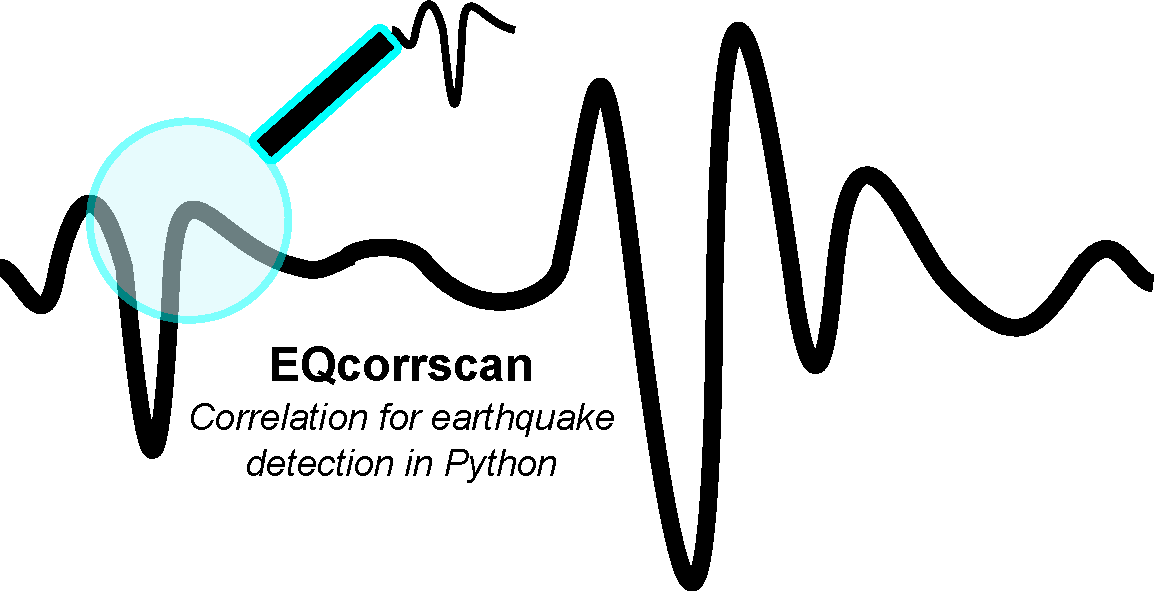
\includegraphics{EQcorrscan_logo.pdf}\par}
\renewcommand{\releasename}{Release}
\makeindex

\makeatletter
\def\PYG@reset{\let\PYG@it=\relax \let\PYG@bf=\relax%
    \let\PYG@ul=\relax \let\PYG@tc=\relax%
    \let\PYG@bc=\relax \let\PYG@ff=\relax}
\def\PYG@tok#1{\csname PYG@tok@#1\endcsname}
\def\PYG@toks#1+{\ifx\relax#1\empty\else%
    \PYG@tok{#1}\expandafter\PYG@toks\fi}
\def\PYG@do#1{\PYG@bc{\PYG@tc{\PYG@ul{%
    \PYG@it{\PYG@bf{\PYG@ff{#1}}}}}}}
\def\PYG#1#2{\PYG@reset\PYG@toks#1+\relax+\PYG@do{#2}}

\expandafter\def\csname PYG@tok@gd\endcsname{\def\PYG@tc##1{\textcolor[rgb]{0.63,0.00,0.00}{##1}}}
\expandafter\def\csname PYG@tok@gu\endcsname{\let\PYG@bf=\textbf\def\PYG@tc##1{\textcolor[rgb]{0.50,0.00,0.50}{##1}}}
\expandafter\def\csname PYG@tok@gt\endcsname{\def\PYG@tc##1{\textcolor[rgb]{0.00,0.27,0.87}{##1}}}
\expandafter\def\csname PYG@tok@gs\endcsname{\let\PYG@bf=\textbf}
\expandafter\def\csname PYG@tok@gr\endcsname{\def\PYG@tc##1{\textcolor[rgb]{1.00,0.00,0.00}{##1}}}
\expandafter\def\csname PYG@tok@cm\endcsname{\let\PYG@it=\textit\def\PYG@tc##1{\textcolor[rgb]{0.25,0.50,0.56}{##1}}}
\expandafter\def\csname PYG@tok@vg\endcsname{\def\PYG@tc##1{\textcolor[rgb]{0.73,0.38,0.84}{##1}}}
\expandafter\def\csname PYG@tok@m\endcsname{\def\PYG@tc##1{\textcolor[rgb]{0.13,0.50,0.31}{##1}}}
\expandafter\def\csname PYG@tok@mh\endcsname{\def\PYG@tc##1{\textcolor[rgb]{0.13,0.50,0.31}{##1}}}
\expandafter\def\csname PYG@tok@cs\endcsname{\def\PYG@tc##1{\textcolor[rgb]{0.25,0.50,0.56}{##1}}\def\PYG@bc##1{\setlength{\fboxsep}{0pt}\colorbox[rgb]{1.00,0.94,0.94}{\strut ##1}}}
\expandafter\def\csname PYG@tok@ge\endcsname{\let\PYG@it=\textit}
\expandafter\def\csname PYG@tok@vc\endcsname{\def\PYG@tc##1{\textcolor[rgb]{0.73,0.38,0.84}{##1}}}
\expandafter\def\csname PYG@tok@il\endcsname{\def\PYG@tc##1{\textcolor[rgb]{0.13,0.50,0.31}{##1}}}
\expandafter\def\csname PYG@tok@go\endcsname{\def\PYG@tc##1{\textcolor[rgb]{0.20,0.20,0.20}{##1}}}
\expandafter\def\csname PYG@tok@cp\endcsname{\def\PYG@tc##1{\textcolor[rgb]{0.00,0.44,0.13}{##1}}}
\expandafter\def\csname PYG@tok@gi\endcsname{\def\PYG@tc##1{\textcolor[rgb]{0.00,0.63,0.00}{##1}}}
\expandafter\def\csname PYG@tok@gh\endcsname{\let\PYG@bf=\textbf\def\PYG@tc##1{\textcolor[rgb]{0.00,0.00,0.50}{##1}}}
\expandafter\def\csname PYG@tok@ni\endcsname{\let\PYG@bf=\textbf\def\PYG@tc##1{\textcolor[rgb]{0.84,0.33,0.22}{##1}}}
\expandafter\def\csname PYG@tok@nl\endcsname{\let\PYG@bf=\textbf\def\PYG@tc##1{\textcolor[rgb]{0.00,0.13,0.44}{##1}}}
\expandafter\def\csname PYG@tok@nn\endcsname{\let\PYG@bf=\textbf\def\PYG@tc##1{\textcolor[rgb]{0.05,0.52,0.71}{##1}}}
\expandafter\def\csname PYG@tok@no\endcsname{\def\PYG@tc##1{\textcolor[rgb]{0.38,0.68,0.84}{##1}}}
\expandafter\def\csname PYG@tok@na\endcsname{\def\PYG@tc##1{\textcolor[rgb]{0.25,0.44,0.63}{##1}}}
\expandafter\def\csname PYG@tok@nb\endcsname{\def\PYG@tc##1{\textcolor[rgb]{0.00,0.44,0.13}{##1}}}
\expandafter\def\csname PYG@tok@nc\endcsname{\let\PYG@bf=\textbf\def\PYG@tc##1{\textcolor[rgb]{0.05,0.52,0.71}{##1}}}
\expandafter\def\csname PYG@tok@nd\endcsname{\let\PYG@bf=\textbf\def\PYG@tc##1{\textcolor[rgb]{0.33,0.33,0.33}{##1}}}
\expandafter\def\csname PYG@tok@ne\endcsname{\def\PYG@tc##1{\textcolor[rgb]{0.00,0.44,0.13}{##1}}}
\expandafter\def\csname PYG@tok@nf\endcsname{\def\PYG@tc##1{\textcolor[rgb]{0.02,0.16,0.49}{##1}}}
\expandafter\def\csname PYG@tok@si\endcsname{\let\PYG@it=\textit\def\PYG@tc##1{\textcolor[rgb]{0.44,0.63,0.82}{##1}}}
\expandafter\def\csname PYG@tok@s2\endcsname{\def\PYG@tc##1{\textcolor[rgb]{0.25,0.44,0.63}{##1}}}
\expandafter\def\csname PYG@tok@vi\endcsname{\def\PYG@tc##1{\textcolor[rgb]{0.73,0.38,0.84}{##1}}}
\expandafter\def\csname PYG@tok@nt\endcsname{\let\PYG@bf=\textbf\def\PYG@tc##1{\textcolor[rgb]{0.02,0.16,0.45}{##1}}}
\expandafter\def\csname PYG@tok@nv\endcsname{\def\PYG@tc##1{\textcolor[rgb]{0.73,0.38,0.84}{##1}}}
\expandafter\def\csname PYG@tok@s1\endcsname{\def\PYG@tc##1{\textcolor[rgb]{0.25,0.44,0.63}{##1}}}
\expandafter\def\csname PYG@tok@gp\endcsname{\let\PYG@bf=\textbf\def\PYG@tc##1{\textcolor[rgb]{0.78,0.36,0.04}{##1}}}
\expandafter\def\csname PYG@tok@sh\endcsname{\def\PYG@tc##1{\textcolor[rgb]{0.25,0.44,0.63}{##1}}}
\expandafter\def\csname PYG@tok@ow\endcsname{\let\PYG@bf=\textbf\def\PYG@tc##1{\textcolor[rgb]{0.00,0.44,0.13}{##1}}}
\expandafter\def\csname PYG@tok@sx\endcsname{\def\PYG@tc##1{\textcolor[rgb]{0.78,0.36,0.04}{##1}}}
\expandafter\def\csname PYG@tok@bp\endcsname{\def\PYG@tc##1{\textcolor[rgb]{0.00,0.44,0.13}{##1}}}
\expandafter\def\csname PYG@tok@c1\endcsname{\let\PYG@it=\textit\def\PYG@tc##1{\textcolor[rgb]{0.25,0.50,0.56}{##1}}}
\expandafter\def\csname PYG@tok@kc\endcsname{\let\PYG@bf=\textbf\def\PYG@tc##1{\textcolor[rgb]{0.00,0.44,0.13}{##1}}}
\expandafter\def\csname PYG@tok@c\endcsname{\let\PYG@it=\textit\def\PYG@tc##1{\textcolor[rgb]{0.25,0.50,0.56}{##1}}}
\expandafter\def\csname PYG@tok@mf\endcsname{\def\PYG@tc##1{\textcolor[rgb]{0.13,0.50,0.31}{##1}}}
\expandafter\def\csname PYG@tok@err\endcsname{\def\PYG@bc##1{\setlength{\fboxsep}{0pt}\fcolorbox[rgb]{1.00,0.00,0.00}{1,1,1}{\strut ##1}}}
\expandafter\def\csname PYG@tok@mb\endcsname{\def\PYG@tc##1{\textcolor[rgb]{0.13,0.50,0.31}{##1}}}
\expandafter\def\csname PYG@tok@ss\endcsname{\def\PYG@tc##1{\textcolor[rgb]{0.32,0.47,0.09}{##1}}}
\expandafter\def\csname PYG@tok@sr\endcsname{\def\PYG@tc##1{\textcolor[rgb]{0.14,0.33,0.53}{##1}}}
\expandafter\def\csname PYG@tok@mo\endcsname{\def\PYG@tc##1{\textcolor[rgb]{0.13,0.50,0.31}{##1}}}
\expandafter\def\csname PYG@tok@kd\endcsname{\let\PYG@bf=\textbf\def\PYG@tc##1{\textcolor[rgb]{0.00,0.44,0.13}{##1}}}
\expandafter\def\csname PYG@tok@mi\endcsname{\def\PYG@tc##1{\textcolor[rgb]{0.13,0.50,0.31}{##1}}}
\expandafter\def\csname PYG@tok@kn\endcsname{\let\PYG@bf=\textbf\def\PYG@tc##1{\textcolor[rgb]{0.00,0.44,0.13}{##1}}}
\expandafter\def\csname PYG@tok@o\endcsname{\def\PYG@tc##1{\textcolor[rgb]{0.40,0.40,0.40}{##1}}}
\expandafter\def\csname PYG@tok@kr\endcsname{\let\PYG@bf=\textbf\def\PYG@tc##1{\textcolor[rgb]{0.00,0.44,0.13}{##1}}}
\expandafter\def\csname PYG@tok@s\endcsname{\def\PYG@tc##1{\textcolor[rgb]{0.25,0.44,0.63}{##1}}}
\expandafter\def\csname PYG@tok@kp\endcsname{\def\PYG@tc##1{\textcolor[rgb]{0.00,0.44,0.13}{##1}}}
\expandafter\def\csname PYG@tok@w\endcsname{\def\PYG@tc##1{\textcolor[rgb]{0.73,0.73,0.73}{##1}}}
\expandafter\def\csname PYG@tok@kt\endcsname{\def\PYG@tc##1{\textcolor[rgb]{0.56,0.13,0.00}{##1}}}
\expandafter\def\csname PYG@tok@sc\endcsname{\def\PYG@tc##1{\textcolor[rgb]{0.25,0.44,0.63}{##1}}}
\expandafter\def\csname PYG@tok@sb\endcsname{\def\PYG@tc##1{\textcolor[rgb]{0.25,0.44,0.63}{##1}}}
\expandafter\def\csname PYG@tok@k\endcsname{\let\PYG@bf=\textbf\def\PYG@tc##1{\textcolor[rgb]{0.00,0.44,0.13}{##1}}}
\expandafter\def\csname PYG@tok@se\endcsname{\let\PYG@bf=\textbf\def\PYG@tc##1{\textcolor[rgb]{0.25,0.44,0.63}{##1}}}
\expandafter\def\csname PYG@tok@sd\endcsname{\let\PYG@it=\textit\def\PYG@tc##1{\textcolor[rgb]{0.25,0.44,0.63}{##1}}}

\def\PYGZbs{\char`\\}
\def\PYGZus{\char`\_}
\def\PYGZob{\char`\{}
\def\PYGZcb{\char`\}}
\def\PYGZca{\char`\^}
\def\PYGZam{\char`\&}
\def\PYGZlt{\char`\<}
\def\PYGZgt{\char`\>}
\def\PYGZsh{\char`\#}
\def\PYGZpc{\char`\%}
\def\PYGZdl{\char`\$}
\def\PYGZhy{\char`\-}
\def\PYGZsq{\char`\'}
\def\PYGZdq{\char`\"}
\def\PYGZti{\char`\~}
% for compatibility with earlier versions
\def\PYGZat{@}
\def\PYGZlb{[}
\def\PYGZrb{]}
\makeatother

\renewcommand\PYGZsq{\textquotesingle}

\begin{document}

\maketitle
\tableofcontents
\phantomsection\label{index::doc}

\href{https://github.com/calum-chamberlain/EQcorrscan/releases}{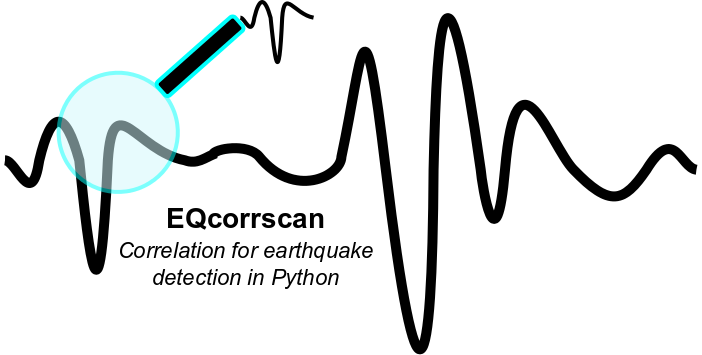
\includegraphics{EQcorrscan_logo.png}}

\chapter{EQcorrscan}
\label{index:eqcorrscan}\label{index:welcome-to-eqcorrscan-s-documentation}
A python package to conduct match-filter earthquake detections.  Codes are stored
on github, the bleeding edge master is \href{https://github.com/calum-chamberlain/EQcorrscan}{here}, or the latest stable(ish) release
can be found \href{https://github.com/calum-chamberlain/EQcorrscan/releases}{here}

This package contains routines to enable the user to conduct match-filter earthquake
detections using \href{https://github.com/obspy/obspy/wiki}{Obspy} bindings when reading
and writing seismic data, and the correlation routine in \href{http://opencv.org/}{openCV}.
Neither of these packages are installed by this software, due to a range of
licences being implimented.  However, both are open-source and should be installed
before using this package.  This package was written to impliment the matlab routines
used by Chamberlain et al. (2014) for the detection of low-frequency earthquakes.

Also within this package are:
\begin{itemize}
\item {} 
Clustering routines for seismic data;

\item {} 
Peak finding algorithm (basic);

\item {} 
Automatic amplitude picker for local magnitude scale;

\item {} 
\href{http://seisan.info/}{Seisan} S-file integration for database management and routine earthquake location;

\item {} 
Stacking routines including phase-weighted stacking based on Thurber at al. (2014);

\item {} 
Brightness based template creation based on the work of Frank et al. (2014)

\end{itemize}

This package is written by Calum Chamberlain of Victoria University of Wellington, and
is distributed under the LGPL GNU Licence, Copyright Calum Chamberlain 2015.


\chapter{References}
\label{index:references}\begin{itemize}
\item {} 
CJ Chamberlain, DR Shelly, J Townend, TA Stern (2014) \href{http://onlinelibrary.wiley.com/doi/10.1002/2014GC005436/full}{Low‐frequency earthquakes reveal punctuated slow slip on the deep extent of the Alpine Fault, New Zealand}, \emph{G-cubed}, doi:10.1002/2014GC005436

\item {} 
Thurber, C. H., Zeng, X., Thomas, A. M., \& Audet, P. (2014). \href{http://www.bssaonline.org/content/early/2014/08/12/0120140077.abstract}{Phase‐Weighted Stacking Applied to Low‐Frequency Earthquakes}, \emph{BSSA}, doi:10.1785/0120140077.

\item {} 
Frank, W. B., \& Shapiro, N. M. (2014). \href{http://gji.oxfordjournals.org/content/197/2/1215.short}{Automatic detection of low-frequency earthquakes (LFEs) based on a beamformed network response}, \emph{Geophysical Journal International}, 197(2), 1215-1223, doi:10.1093/gji/ggu058.

\end{itemize}


\chapter{Contents:}
\label{index:contents}

\section{Introduction to the EQcorrscan package}
\label{intro:introduction-to-the-eqcorrscan-package}\label{intro::doc}
This document is designed to give you an overview of the capabilities and
implimentation of the EQcorrscan python module.


\subsection{Installation}
\label{intro:installation}
Most codes should work without any effort on your part.  However you must
install the packages this package relies on yourself, this includes the follwing
packages:
\begin{itemize}
\item {} 
matplotlib

\item {} 
numpy

\item {} 
scipy

\item {} 
obspy

\item {} 
joblib

\item {} 
openCV (2)

\end{itemize}

This install has only been tested on Linux machines and even then has some
issues when installing on 32-Bit versus 64-Bit machines.  In this instance you
should be prepared for small differences in the results of your correlations
relating to foating-point truncation differences between 32 and 64-Bit
machines.

If you plan to run the bright\_lights.py routines you will need to have
NonLinLoc installed on your machine.  This is not provided here and should
be sourced from \href{http://alomax.free.fr/nlloc/}{NonLinLoc} This will provide
the Grid2Time routine which is required to set-up a lag-time grid for your
velocity model.  You should read the NonLinLoc documentation for more
information regarding how this process works and the input files you are
required to give.


\subsection{Functions}
\label{intro:functions}
This package is divided into sub-directories of \emph{core}, \emph{par} and \emph{utils}.  The
\emph{utils} directory contains simple functions for integration with
\href{http://seisan.info/}{seisan}, these is the \emph{Sfile\_util.py}
module and functions therein which are essentially barebones and do not have the
full functionality that seisan can handle.  \emph{utils} also contains a simple
peak-finding algorithm \emph{find\_peaks.py} which looks for peaks within noisy data
above a certain threshold and within windows.

Within \emph{par} you will find parameter files which you will need to edit for
each of the \emph{core} scripts.  \emph{core} scripts often call on multiple \emph{par} files
so be sure to set them all up.  The \emph{template\_gen\_par.py} script is used by all
\emph{core} modules and must be set-up.  Within this you will define all your
template parameters.  Currently the templates must all be of the same length,
but this may change in a future release.

Within \emph{core} you will find the core routines to generate templates,
\emph{(template\_gen.py)} search for likely templates \emph{(bright\_lights.py)} and
compute cross-channel correlations from these templates \emph{(match\_filter.py)}.


\section{EQcorrscan tutorial}
\label{tutorial:eqcorrscan-tutorial}\label{tutorial::doc}
Welcome to EQcorrscan - this package is designed to compute earthquake detections
using a paralleled match-filter network cross-correlation routine.  The inner
loop of this package is the cross-correaltion of templates of seismic data
with daylong seismic data.  This inner function is the openCV.match\_template
function - this appears to be a well optimized cross-correlation function written
in c++.  Cross-correlations are computed in the frequency domain for large
datasets, for which a day of seismic data usually qualifies.

Before continuing with this tutorial please check that you have installed all
the pre-requisite modules, as this won't be done for you.  The list of these is
in the Introduction section of this documentation.

As you will see, this package is divided into three main sub-modules, the
Core, Utils and Par sub-modules.  The Core sub-module contains the main, high-level
functions:
\begin{quote}\begin{description}
\item[{bright\_lights}] \leavevmode
A brightness based template detection routine;

\item[{template\_gen}] \leavevmode
A series of routines to generate templates for match-filter detection
from continuous or cut data, with pick-times defined either manually, or from a
\emph{Seian} s-file;

\item[{match\_filter}] \leavevmode
The main match-filter routines, this is split into several
smaller functions to allow python based parallelisation;

\item[{lag\_calc}] \leavevmode
Routines for calculating optimal lag-times for events detected
by the match-filter routine, these lags can then be used to define new picks
for high accuracy reloactions.

\end{description}\end{quote}

The Par sub-module contains parameter files which are provided to allow for simple
bulk processing of large datasets.  These \emph{MUST} be edited by the user for their
dataset.

The Utils sub-module contains useful, but small functions.  These functions are
rarely cpu intensive, but perform vital operations, such as reading \emph{Seisan} s-files,
finding peaks in noisy data, converting a seisan database to hypoDD formatted
files and computing cross-correlations between detections for hypoDD (a double
difference reloaction software), calculating magnitudes, clustering detections,
stacking detections, making pretty plots, and processing seismic data in the
same way repeatedly using \emph{Obspy}`s functionality.


\subsection{Match-filter detection}
\label{tutorial:match-filter-detection}
In this section we will discuss generating a template from a \emph{Seisan} s-file, and
using this template to scan for similar earthquakes within a day of data.  This single
template and single day of data does not truely exploit the parallel operations within
this package however, so you would be encouraged to think about where parallel operations
occur (\emph{hint, the code can run one template per cpu}), and why there are --instance and
--splits flags (\emph{hint, if you have heaps of memory and cpus you can do some brute
force day parallelisation!}).

The following script is included in the top-level directory alongside the full-scripts
used by the author to generate a 6.5 year long catalogue of low-frequency earthquakes
for the central Southern Alps of New Zealand.

This tutorial script highlights the ability of the match-filter method in detecting
earthquakes of near-repeating nature.  The dataset is a day of data taken from the
New Zealand national database, and the Southern Alp Microearthquake Borehole Array
(SAMBA) network (Boese et al. 2012).  This day was found to contain a swarm of
earthquakes, as published by Boese et al. (2014), the s-file provided is one of
these events.

The main processing flow is outlined in the figure below, note the main speedups
in this process are achioeved by running multiple templates at once, however this
increaces memory usage.  If memory is problem there are flags (mem\_issue) in the
match\_filter.py source that can be turned on - the codes will then write temporary
files, which is slower, but can allow for more data crunching at once, your trade-off,
your call.

{\hfill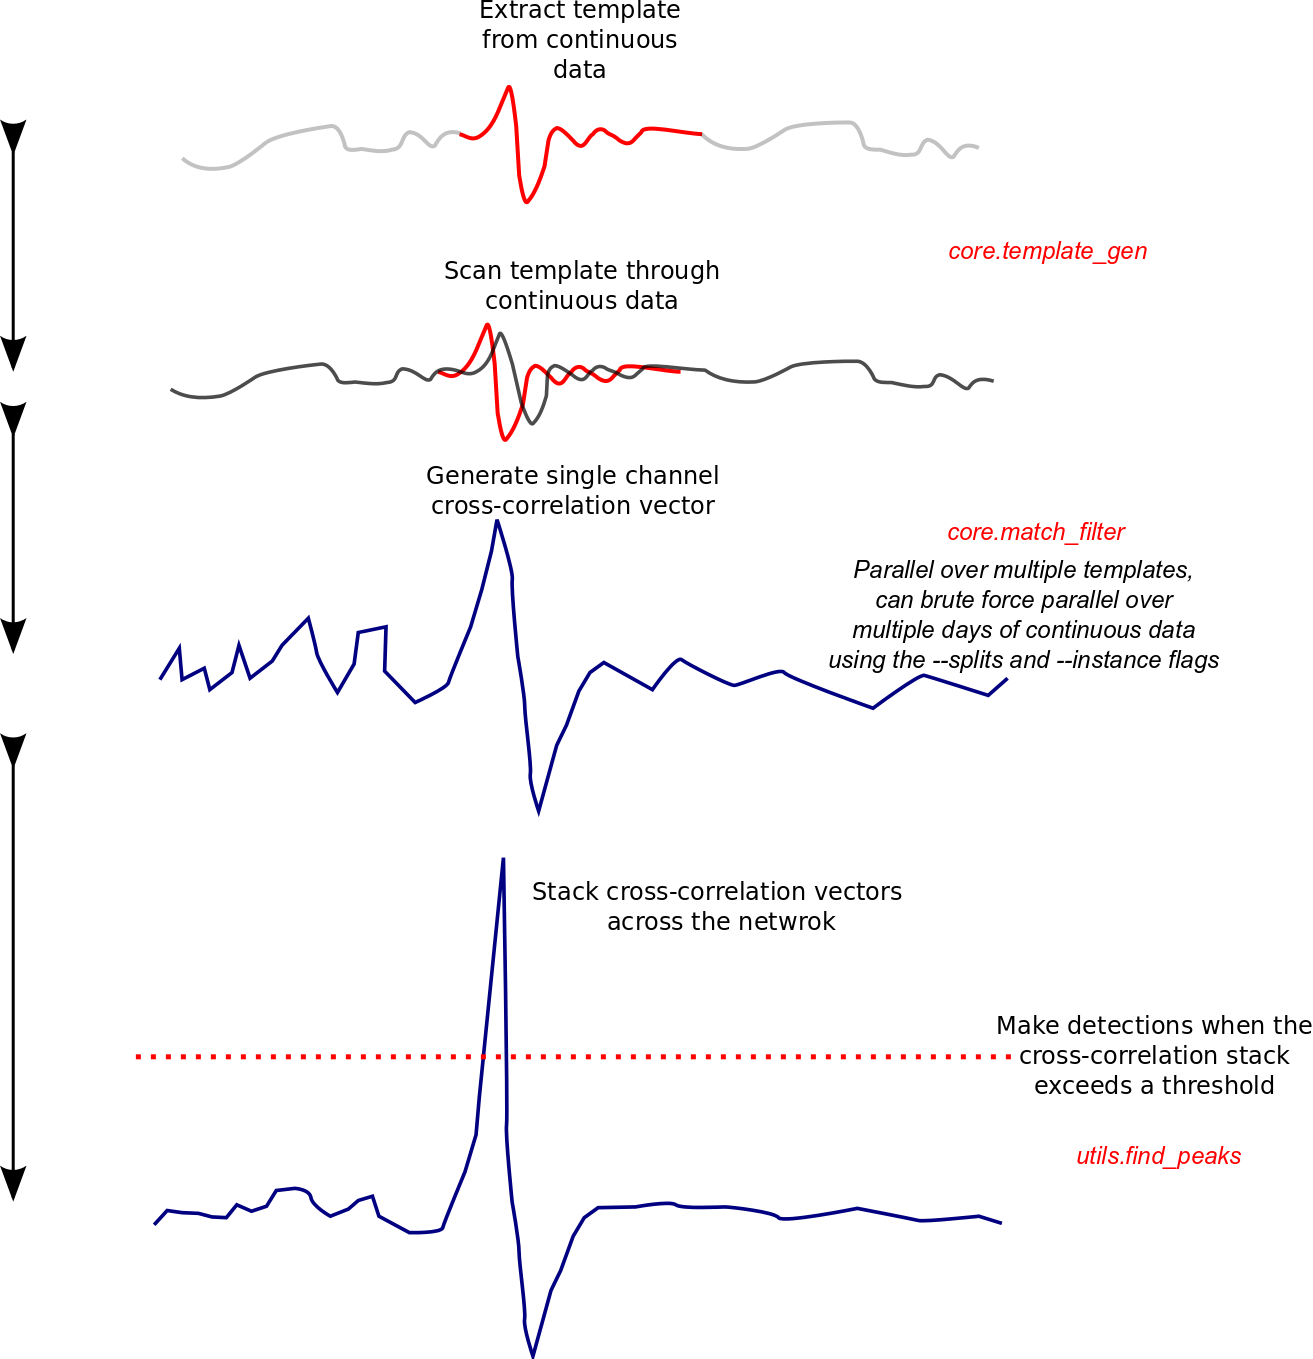
\includegraphics{processing_flow.png}\hfill}


\subsection{References}
\label{tutorial:references}\begin{itemize}
\item {} 
CM Boese, J Townend, E Smith, T Stern (2012). \href{http://onlinelibrary.wiley.com/doi/10.1029/2011JB008460/full}{Microseismicity and stress in the vicinity of the Alpine Fault, central Southern Alps, New Zealand}, \emph{JGR}, doi:10.1029/2011JB008460

\item {} 
CM Boese, KM Jacobs, EGC Smith, TA Stern, J Townend (2014). \href{http://onlinelibrary.wiley.com/doi/10.1002/2013GC005171/full}{Background and delayed-triggered swarms in the central Southern Alps, South Island, New Zealand}, \emph{G-cubed}, doi:10.1002/2013GC005171

\end{itemize}

\begin{Verbatim}[commandchars=\\\{\}]
\PYG{c}{\PYGZsh{}!/usr/bin/python}
\PYG{l+s+sd}{\PYGZdq{}\PYGZdq{}\PYGZdq{}}
\PYG{l+s+sd}{Tutorial}

\PYG{l+s+sd}{    This script is designed as a tutorial to highlight how to call the main}
\PYG{l+s+sd}{    functions within the EQcorrscan module.  In this tutorial we will see how}
\PYG{l+s+sd}{    to generate a template and run this through the match\PYGZhy{}filter routine.}

\PYG{l+s+sd}{    The template will be generated from a pre\PYGZhy{}picked earthquake, however there}
\PYG{l+s+sd}{    are other ways to generate templates, for example this package also contains}
\PYG{l+s+sd}{    a simple brightness function that is designed to scan continuous seismic}
\PYG{l+s+sd}{    data and look for impulsive energy originating from a discrete point in a}
\PYG{l+s+sd}{    seismic velocity model.  The use of this brightness function is not}
\PYG{l+s+sd}{    included in this tutorial script yet because it is still in beta.}

\PYG{l+s+sd}{This package is dstributed under the LGPL v3.0, by using this script and the}
\PYG{l+s+sd}{functions contained within the EQcorrscan package you implicitly accept the}
\PYG{l+s+sd}{licence.  For the full wording of the licence refer to the licence.txt file.}

\PYG{l+s+sd}{Copyright 2015 Calum Chamberlain}

\PYG{l+s+sd}{This file is part of EQcorrscan.}

\PYG{l+s+sd}{    EQcorrscan is free software: you can redistribute it and/or modify}
\PYG{l+s+sd}{    it under the terms of the GNU General Public License as published by}
\PYG{l+s+sd}{    the Free Software Foundation, either version 3 of the License, or}
\PYG{l+s+sd}{    (at your option) any later version.}

\PYG{l+s+sd}{    EQcorrscan is distributed in the hope that it will be useful,}
\PYG{l+s+sd}{    but WITHOUT ANY WARRANTY; without even the implied warranty of}
\PYG{l+s+sd}{    MERCHANTABILITY or FITNESS FOR A PARTICULAR PURPOSE.  See the}
\PYG{l+s+sd}{    GNU General Public License for more details.}

\PYG{l+s+sd}{    You should have received a copy of the GNU General Public License}
\PYG{l+s+sd}{    along with EQcorrscan.  If not, see \PYGZlt{}http://www.gnu.org/licenses/\PYGZgt{}.}

\PYG{l+s+sd}{\PYGZdq{}\PYGZdq{}\PYGZdq{}}

\PYG{c}{\PYGZsh{} First we import the required modules:}
\PYG{k+kn}{from} \PYG{n+nn}{obspy} \PYG{k+kn}{import} \PYG{n}{read}\PYG{p}{,} \PYG{n}{Stream}
\PYG{k+kn}{from} \PYG{n+nn}{core} \PYG{k+kn}{import} \PYG{n}{template\PYGZus{}gen}\PYG{p}{,} \PYG{n}{match\PYGZus{}filter}
\PYG{k+kn}{from} \PYG{n+nn}{par} \PYG{k+kn}{import} \PYG{n}{template\PYGZus{}gen\PYGZus{}par} \PYG{k}{as} \PYG{n}{templatedef}
\PYG{k+kn}{from} \PYG{n+nn}{par} \PYG{k+kn}{import} \PYG{n}{match\PYGZus{}filter\PYGZus{}par} \PYG{k}{as} \PYG{n}{matchdef}
\PYG{k+kn}{from} \PYG{n+nn}{utils} \PYG{k+kn}{import} \PYG{n}{pre\PYGZus{}processing}\PYG{p}{,} \PYG{n}{Sfile\PYGZus{}util}
\PYG{k+kn}{import} \PYG{n+nn}{glob}

\PYG{c}{\PYGZsh{} Now we find the s\PYGZhy{}file we want to use to generate a template from}
\PYG{n}{sfiles}\PYG{o}{=}\PYG{n}{glob}\PYG{o}{.}\PYG{n}{glob}\PYG{p}{(}\PYG{l+s}{\PYGZsq{}}\PYG{l+s}{test\PYGZus{}data/tutorial\PYGZus{}data/*L.S*}\PYG{l+s}{\PYGZsq{}}\PYG{p}{)}

\PYG{c}{\PYGZsh{} Generate the template from these sfiles:}
\PYG{n}{templates}\PYG{o}{=}\PYG{p}{[}\PYG{p}{]} \PYG{c}{\PYGZsh{} Open a list to be filled \PYGZhy{} only applies for multiple templates}
\PYG{n}{template\PYGZus{}names}\PYG{o}{=}\PYG{p}{[}\PYG{p}{]} \PYG{c}{\PYGZsh{} List of template names for later ID}
\PYG{n}{i}\PYG{o}{=}\PYG{l+m+mi}{0} \PYG{c}{\PYGZsh{} Template name iterator}
\PYG{k}{for} \PYG{n}{sfile} \PYG{o+ow}{in} \PYG{n}{sfiles}\PYG{p}{:}
    \PYG{c}{\PYGZsh{} Read in the picks from the S\PYGZhy{}file, note, in the full case one fo the main\PYGZbs{}}
            \PYG{c}{\PYGZsh{} functions in template\PYGZus{}gen would be used rather than this, but for\PYGZbs{}}
            \PYG{c}{\PYGZsh{} the tutorial we will read in the data here \PYGZhy{} also note that this\PYGZbs{}}
            \PYG{c}{\PYGZsh{} template generation is inefficient for multiple templates, if using\PYGZbs{}}
            \PYG{c}{\PYGZsh{} daylong data for multiple templates you would want to only read\PYGZbs{}}
            \PYG{c}{\PYGZsh{} the seismic data once and cut it multiple times.}
    \PYG{n}{picks}\PYG{o}{=}\PYG{n}{Sfile\PYGZus{}util}\PYG{o}{.}\PYG{n}{readpicks}\PYG{p}{(}\PYG{n}{sfile}\PYG{p}{)}
    \PYG{k}{for} \PYG{n}{pick} \PYG{o+ow}{in} \PYG{n}{picks}\PYG{p}{:}
        \PYG{k}{if} \PYG{o+ow}{not} \PYG{l+s}{\PYGZsq{}}\PYG{l+s}{wavefiles}\PYG{l+s}{\PYGZsq{}} \PYG{o+ow}{in} \PYG{n+nb}{locals}\PYG{p}{(}\PYG{p}{)}\PYG{p}{:}
            \PYG{n}{wavefiles}\PYG{o}{=}\PYG{n}{glob}\PYG{o}{.}\PYG{n}{glob}\PYG{p}{(}\PYG{l+s}{\PYGZsq{}}\PYG{l+s}{test\PYGZus{}data/tutorial\PYGZus{}data/}\PYG{l+s}{\PYGZsq{}}\PYG{o}{+}\PYGZbs{}
                                   \PYG{n}{pick}\PYG{o}{.}\PYG{n}{station}\PYG{o}{+}\PYG{l+s}{\PYGZsq{}}\PYG{l+s}{.*}\PYG{l+s}{\PYGZsq{}}\PYG{p}{)}
        \PYG{k}{else}\PYG{p}{:}
            \PYG{n}{wavefiles}\PYG{o}{+}\PYG{o}{=}\PYG{n}{glob}\PYG{o}{.}\PYG{n}{glob}\PYG{p}{(}\PYG{l+s}{\PYGZsq{}}\PYG{l+s}{test\PYGZus{}data/tutorial\PYGZus{}data/}\PYG{l+s}{\PYGZsq{}}\PYG{o}{+}\PYGZbs{}
                                 \PYG{n}{pick}\PYG{o}{.}\PYG{n}{station}\PYG{o}{+}\PYG{l+s}{\PYGZsq{}}\PYG{l+s}{.*}\PYG{l+s}{\PYGZsq{}}\PYG{p}{)}
    \PYG{n}{wavefiles}\PYG{o}{=}\PYG{n+nb}{list}\PYG{p}{(}\PYG{n+nb}{set}\PYG{p}{(}\PYG{n}{wavefiles}\PYG{p}{)}\PYG{p}{)}
    \PYG{k}{for} \PYG{n}{wavefile} \PYG{o+ow}{in} \PYG{n}{wavefiles}\PYG{p}{:}
        \PYG{k}{print} \PYG{l+s}{\PYGZsq{}}\PYG{l+s}{Reading data from }\PYG{l+s}{\PYGZsq{}}\PYG{o}{+}\PYG{n}{wavefile}
        \PYG{k}{if} \PYG{o+ow}{not} \PYG{l+s}{\PYGZsq{}}\PYG{l+s}{st}\PYG{l+s}{\PYGZsq{}} \PYG{o+ow}{in} \PYG{n+nb}{locals}\PYG{p}{(}\PYG{p}{)}\PYG{p}{:}
            \PYG{n}{st}\PYG{o}{=}\PYG{n}{read}\PYG{p}{(}\PYG{n}{wavefile}\PYG{p}{)}
        \PYG{k}{else}\PYG{p}{:}
            \PYG{n}{st}\PYG{o}{+}\PYG{o}{=}\PYG{n}{read}\PYG{p}{(}\PYG{n}{wavefile}\PYG{p}{)}
    \PYG{n}{st}\PYG{o}{=}\PYG{n}{st}\PYG{o}{.}\PYG{n}{merge}\PYG{p}{(}\PYG{n}{fill\PYGZus{}value}\PYG{o}{=}\PYG{l+s}{\PYGZsq{}}\PYG{l+s}{interpolate}\PYG{l+s}{\PYGZsq{}}\PYG{p}{)}
    \PYG{n}{day}\PYG{o}{=}\PYG{n}{st}\PYG{p}{[}\PYG{l+m+mi}{0}\PYG{p}{]}\PYG{o}{.}\PYG{n}{stats}\PYG{o}{.}\PYG{n}{starttime}\PYG{o}{.}\PYG{n}{date}
    \PYG{k}{for} \PYG{n}{tr} \PYG{o+ow}{in} \PYG{n}{st}\PYG{p}{:}
        \PYG{n}{tr}\PYG{o}{=}\PYG{n}{pre\PYGZus{}processing}\PYG{o}{.}\PYG{n}{dayproc}\PYG{p}{(}\PYG{n}{tr}\PYG{p}{,} \PYG{l+m+mf}{1.0}\PYG{p}{,} \PYG{l+m+mf}{20.0}\PYG{p}{,} \PYG{l+m+mi}{3}\PYG{p}{,} \PYG{l+m+mf}{100.0}\PYG{p}{,}\PYGZbs{}
                                  \PYG{n}{matchdef}\PYG{o}{.}\PYG{n}{debug}\PYG{p}{,} \PYG{n}{day}\PYG{p}{)}
    \PYG{c}{\PYGZsh{} Apply a small amoutn of delay before the pick}
    \PYG{k}{for} \PYG{n}{pick} \PYG{o+ow}{in} \PYG{n}{picks}\PYG{p}{:}
        \PYG{n}{pick}\PYG{o}{.}\PYG{n}{time}\PYG{o}{=}\PYG{n}{pick}\PYG{o}{.}\PYG{n}{time}\PYG{o}{\PYGZhy{}}\PYG{l+m+mf}{0.1}
    \PYG{n}{template}\PYG{o}{=}\PYG{n}{template\PYGZus{}gen}\PYG{o}{.}\PYG{n}{\PYGZus{}template\PYGZus{}gen}\PYG{p}{(}\PYG{n}{picks}\PYG{p}{,} \PYG{n}{st}\PYG{p}{,} \PYG{l+m+mf}{1.0}\PYG{p}{,} \PYG{l+s}{\PYGZsq{}}\PYG{l+s}{all}\PYG{l+s}{\PYGZsq{}}\PYG{p}{)}
    \PYG{c}{\PYGZsh{} This will generate an obspy.Stream object}
    \PYG{c}{\PYGZsh{} Append this Stream to the list of templates}
    \PYG{n}{templates}\PYG{o}{+}\PYG{o}{=}\PYG{p}{[}\PYG{n}{template}\PYG{p}{]}
    \PYG{n}{template\PYGZus{}names}\PYG{o}{.}\PYG{n}{append}\PYG{p}{(}\PYG{l+s}{\PYGZsq{}}\PYG{l+s}{tutorial\PYGZus{}}\PYG{l+s}{\PYGZsq{}}\PYG{o}{+}\PYG{n+nb}{str}\PYG{p}{(}\PYG{n}{i}\PYG{p}{)}\PYG{p}{)}
    \PYG{c}{\PYGZsh{} Plot the template just to check that all is well!}
    \PYG{n}{template}\PYG{o}{.}\PYG{n}{plot}\PYG{p}{(}\PYG{n}{size}\PYG{o}{=}\PYG{p}{(}\PYG{l+m+mi}{800}\PYG{p}{,}\PYG{l+m+mi}{600}\PYG{p}{)}\PYG{p}{,} \PYG{n}{equal\PYGZus{}scale}\PYG{o}{=}\PYG{n+nb+bp}{False}\PYG{p}{)}
    \PYG{c}{\PYGZsh{} Save template for later}
    \PYG{n}{template}\PYG{o}{.}\PYG{n}{write}\PYG{p}{(}\PYG{l+s}{\PYGZsq{}}\PYG{l+s}{test\PYGZus{}data/tutorial\PYGZus{}data/}\PYG{l+s}{\PYGZsq{}}\PYG{o}{+}\PYG{n}{template\PYGZus{}names}\PYG{p}{[}\PYG{n}{i}\PYG{p}{]}\PYG{o}{+}\PYG{l+s}{\PYGZsq{}}\PYG{l+s}{\PYGZus{}template.ms}\PYG{l+s}{\PYGZsq{}}\PYG{p}{,}\PYGZbs{}
                   \PYG{n}{format}\PYG{o}{=}\PYG{l+s}{\PYGZsq{}}\PYG{l+s}{MSEED}\PYG{l+s}{\PYGZsq{}}\PYG{p}{)}
    \PYG{n}{i}\PYG{o}{+}\PYG{o}{=}\PYG{l+m+mi}{1}
    \PYG{k}{del} \PYG{n}{template}\PYG{p}{,} \PYG{n}{st}

\PYG{c}{\PYGZsh{} Extract the stations from the templates}
\PYG{k}{for} \PYG{n}{template} \PYG{o+ow}{in} \PYG{n}{templates}\PYG{p}{:}
    \PYG{k}{if} \PYG{o+ow}{not} \PYG{l+s}{\PYGZsq{}}\PYG{l+s}{stachans}\PYG{l+s}{\PYGZsq{}} \PYG{o+ow}{in} \PYG{n+nb}{locals}\PYG{p}{(}\PYG{p}{)}\PYG{p}{:}
        \PYG{n}{stachans}\PYG{o}{=}\PYG{p}{[}\PYG{p}{(}\PYG{n}{tr}\PYG{o}{.}\PYG{n}{stats}\PYG{o}{.}\PYG{n}{station}\PYG{p}{,} \PYG{n}{tr}\PYG{o}{.}\PYG{n}{stats}\PYG{o}{.}\PYG{n}{channel}\PYG{p}{)} \PYG{k}{for} \PYG{n}{tr} \PYG{o+ow}{in} \PYG{n}{template}\PYG{p}{]}
    \PYG{k}{else}\PYG{p}{:}
        \PYG{n}{stachans}\PYG{o}{+}\PYG{o}{=}\PYG{p}{[}\PYG{p}{(}\PYG{n}{tr}\PYG{o}{.}\PYG{n}{stats}\PYG{o}{.}\PYG{n}{station}\PYG{p}{,} \PYG{n}{tr}\PYG{o}{.}\PYG{n}{stats}\PYG{o}{.}\PYG{n}{channel}\PYG{p}{)} \PYG{k}{for} \PYG{n}{tr} \PYG{o+ow}{in} \PYG{n}{template}\PYG{p}{]}

\PYG{c}{\PYGZsh{} Make this a unique list}
\PYG{n}{stachans}\PYG{o}{=}\PYG{n+nb}{list}\PYG{p}{(}\PYG{n+nb}{set}\PYG{p}{(}\PYG{n}{stachans}\PYG{p}{)}\PYG{p}{)}

\PYG{c}{\PYGZsh{} Read in the continuous data for these station, channel combinations}
\PYG{k}{for} \PYG{n}{stachan} \PYG{o+ow}{in} \PYG{n}{stachans}\PYG{p}{:}
    \PYG{k}{print} \PYG{l+s}{\PYGZsq{}}\PYG{l+s}{Reading data from: test\PYGZus{}data/tutorial\PYGZus{}data/}\PYG{l+s}{\PYGZsq{}}\PYG{o}{+}\PYG{n}{stachan}\PYG{p}{[}\PYG{l+m+mi}{0}\PYG{p}{]}\PYG{o}{+}\PYG{l+s}{\PYGZsq{}}\PYG{l+s}{.*..*}\PYG{l+s}{\PYGZsq{}}\PYG{o}{+}\PYG{n}{stachan}\PYG{p}{[}\PYG{l+m+mi}{1}\PYG{p}{]}\PYG{p}{[}\PYG{o}{\PYGZhy{}}\PYG{l+m+mi}{1}\PYG{p}{]}\PYG{o}{+}\PYG{l+s}{\PYGZsq{}}\PYG{l+s}{.*}\PYG{l+s}{\PYGZsq{}}
    \PYG{c}{\PYGZsh{} Generate a new stream object and add to it}
    \PYG{k}{if} \PYG{o+ow}{not} \PYG{l+s}{\PYGZsq{}}\PYG{l+s}{st}\PYG{l+s}{\PYGZsq{}} \PYG{o+ow}{in} \PYG{n+nb}{locals}\PYG{p}{(}\PYG{p}{)}\PYG{p}{:}
        \PYG{n}{st}\PYG{o}{=}\PYG{n}{read}\PYG{p}{(}\PYG{l+s}{\PYGZsq{}}\PYG{l+s}{test\PYGZus{}data/tutorial\PYGZus{}data/}\PYG{l+s}{\PYGZsq{}}\PYG{o}{+}\PYG{n}{stachan}\PYG{p}{[}\PYG{l+m+mi}{0}\PYG{p}{]}\PYG{o}{+}\PYG{l+s}{\PYGZsq{}}\PYG{l+s}{.*..*}\PYG{l+s}{\PYGZsq{}}\PYG{o}{+}\PYG{n}{stachan}\PYG{p}{[}\PYG{l+m+mi}{1}\PYG{p}{]}\PYG{p}{[}\PYG{o}{\PYGZhy{}}\PYG{l+m+mi}{1}\PYG{p}{]}\PYG{o}{+}\PYG{l+s}{\PYGZsq{}}\PYG{l+s}{.*}\PYG{l+s}{\PYGZsq{}}\PYG{p}{)}
    \PYG{k}{else}\PYG{p}{:}
        \PYG{n}{st}\PYG{o}{+}\PYG{o}{=}\PYG{n}{read}\PYG{p}{(}\PYG{l+s}{\PYGZsq{}}\PYG{l+s}{test\PYGZus{}data/tutorial\PYGZus{}data/}\PYG{l+s}{\PYGZsq{}}\PYG{o}{+}\PYG{n}{stachan}\PYG{p}{[}\PYG{l+m+mi}{0}\PYG{p}{]}\PYG{o}{+}\PYG{l+s}{\PYGZsq{}}\PYG{l+s}{.*..*}\PYG{l+s}{\PYGZsq{}}\PYG{o}{+}\PYG{n}{stachan}\PYG{p}{[}\PYG{l+m+mi}{1}\PYG{p}{]}\PYG{p}{[}\PYG{o}{\PYGZhy{}}\PYG{l+m+mi}{1}\PYG{p}{]}\PYG{o}{+}\PYG{l+s}{\PYGZsq{}}\PYG{l+s}{.*}\PYG{l+s}{\PYGZsq{}}\PYG{p}{)}

\PYG{c}{\PYGZsh{} Merge the data to account for miniseed files being written in chunks}
\PYG{c}{\PYGZsh{} We need continuous day\PYGZhy{}long data, so data are padded if there are gaps}
\PYG{n}{st}\PYG{o}{=}\PYG{n}{st}\PYG{o}{.}\PYG{n}{merge}\PYG{p}{(}\PYG{n}{fill\PYGZus{}value}\PYG{o}{=}\PYG{l+s}{\PYGZsq{}}\PYG{l+s}{interpolate}\PYG{l+s}{\PYGZsq{}}\PYG{p}{)}

\PYG{c}{\PYGZsh{} Work out what day we are working on, required as we will pad the data to be daylong}
\PYG{n}{day}\PYG{o}{=}\PYG{n}{st}\PYG{p}{[}\PYG{l+m+mi}{0}\PYG{p}{]}\PYG{o}{.}\PYG{n}{stats}\PYG{o}{.}\PYG{n}{starttime}\PYG{o}{.}\PYG{n}{date}

\PYG{c}{\PYGZsh{} Process the data in the same way as the template}
\PYG{k}{for} \PYG{n}{tr} \PYG{o+ow}{in} \PYG{n}{st}\PYG{p}{:}
    \PYG{n}{tr}\PYG{o}{=}\PYG{n}{pre\PYGZus{}processing}\PYG{o}{.}\PYG{n}{dayproc}\PYG{p}{(}\PYG{n}{tr}\PYG{p}{,} \PYG{l+m+mf}{1.0}\PYG{p}{,} \PYG{l+m+mf}{20.0}\PYG{p}{,} \PYG{l+m+mi}{3}\PYG{p}{,} \PYG{l+m+mf}{100.0}\PYG{p}{,}\PYGZbs{}
                              \PYG{n}{matchdef}\PYG{o}{.}\PYG{n}{debug}\PYG{p}{,} \PYG{n}{day}\PYG{p}{)}

\PYG{c}{\PYGZsh{} Compute detections}
\PYG{n}{detections}\PYG{o}{=}\PYG{n}{match\PYGZus{}filter}\PYG{o}{.}\PYG{n}{match\PYGZus{}filter}\PYG{p}{(}\PYG{n}{template\PYGZus{}names}\PYG{p}{,} \PYG{n}{templates}\PYG{p}{,} \PYG{n}{st}\PYG{p}{,}\PYGZbs{}
                                     \PYG{n}{matchdef}\PYG{o}{.}\PYG{n}{threshold}\PYG{p}{,} \PYG{n}{matchdef}\PYG{o}{.}\PYG{n}{threshtype}\PYG{p}{,}\PYGZbs{}
                                     \PYG{n}{matchdef}\PYG{o}{.}\PYG{n}{trig\PYGZus{}int}\PYG{p}{,} \PYG{n+nb+bp}{True}\PYG{p}{,}\PYGZbs{}
                                     \PYG{l+s}{\PYGZsq{}}\PYG{l+s}{temp\PYGZus{}0}\PYG{l+s}{\PYGZsq{}}\PYG{p}{)}

\PYG{c}{\PYGZsh{} We now have a list of detections! We can output these to a file to check later}
\PYG{n}{f}\PYG{o}{=}\PYG{n+nb}{open}\PYG{p}{(}\PYG{l+s}{\PYGZsq{}}\PYG{l+s}{tutorial\PYGZus{}detections.csv}\PYG{l+s}{\PYGZsq{}}\PYG{p}{,}\PYG{l+s}{\PYGZsq{}}\PYG{l+s}{w}\PYG{l+s}{\PYGZsq{}}\PYG{p}{)}
\PYG{k}{for} \PYG{n}{detection} \PYG{o+ow}{in} \PYG{n}{detections}\PYG{p}{:}
    \PYG{n}{f}\PYG{o}{.}\PYG{n}{write}\PYG{p}{(}\PYG{n}{detection}\PYG{o}{.}\PYG{n}{template\PYGZus{}name}\PYG{o}{+}\PYG{l+s}{\PYGZsq{}}\PYG{l+s}{, }\PYG{l+s}{\PYGZsq{}}\PYG{o}{+}\PYG{n+nb}{str}\PYG{p}{(}\PYG{n}{detection}\PYG{o}{.}\PYG{n}{detect\PYGZus{}time}\PYG{p}{)}\PYG{o}{+}\PYGZbs{}
            \PYG{l+s}{\PYGZsq{}}\PYG{l+s}{, }\PYG{l+s}{\PYGZsq{}}\PYG{o}{+}\PYG{n+nb}{str}\PYG{p}{(}\PYG{n}{detection}\PYG{o}{.}\PYG{n}{detect\PYGZus{}val}\PYG{p}{)}\PYG{o}{+}\PYG{l+s}{\PYGZsq{}}\PYG{l+s}{, }\PYG{l+s}{\PYGZsq{}}\PYG{o}{+}\PYG{n+nb}{str}\PYG{p}{(}\PYG{n}{detection}\PYG{o}{.}\PYG{n}{threshold}\PYG{p}{)}\PYG{o}{+}\PYGZbs{}
            \PYG{l+s}{\PYGZsq{}}\PYG{l+s}{, }\PYG{l+s}{\PYGZsq{}}\PYG{o}{+}\PYG{n+nb}{str}\PYG{p}{(}\PYG{n}{detection}\PYG{o}{.}\PYG{n}{no\PYGZus{}chans}\PYG{p}{)}\PYG{o}{+}\PYG{l+s}{\PYGZsq{}}\PYG{l+s+se}{\PYGZbs{}n}\PYG{l+s}{\PYGZsq{}}\PYG{p}{)}
\PYG{n}{f}\PYG{o}{.}\PYG{n}{close}\PYG{p}{(}\PYG{p}{)}
\end{Verbatim}


\section{Core}
\label{core:core}\label{core::doc}
Core programs for the EQcorrscan project.


\subsection{bright\_lights}
\label{core:bright-lights}\label{core:module-bright_lights}\index{bright\_lights (module)}
Code to determine the birghtness function of seismic data according to a three-dimensional travel-time grid.  This travel-time grid should be generated usingthe grid2time function of the NonLinLoc package by Anthony Lomax which can befound here: \href{http://alomax.free.fr/nlloc/}{http://alomax.free.fr/nlloc/} and is not distributed within thispackage as this is a very useful stand-alone library for seismic event location.

This code is based on the method of Frank \& Shapiro 2014

Part of the EQcorrscan module to integrate seisan nordic files into a fullcross-channel correlation for detection routine.EQcorrscan is a python module designed to run match filter routines forseismology, within it are routines for integration to seisan and obspy.With obspy integration (which is necessary) all main waveform formats can beread in and output.

This main section contains a script, LFE\_search.py which demonstrates the usageof the built in functions from template generation from picked waveformsthrough detection by match filter of continuous data to the generation of lagtimes to be used for relative locations.

The match-filter routine described here was used a previous Matlab code for theChamberlain et al. 2014 G-cubed publication.  The basis for the lag-timegeneration section is outlined in Hardebeck \& Shelly 2011, GRL.
Code generated by Calum John Chamberlain of Victoria University of Wellington,2015.
\paragraph{Note}
\begin{description}
\item[{Pre-requisites:}] \leavevmode\begin{itemize}
\item {} 
gcc             - for the installation of the openCV correlation routine

\item {} 
python-cv2      - Python bindings for the openCV routines

\item {} 
python-joblib   - used for parallel processing

\item {} \begin{description}
\item[{python-obspy    - used for lots of common seismological processing}] \leavevmode\begin{itemize}
\item {} \begin{description}
\item[{requires:}] \leavevmode\begin{itemize}
\item {} 
numpy

\item {} 
scipy

\item {} 
matplotlib

\end{itemize}

\end{description}

\end{itemize}

\end{description}

\item {} 
NonLinLoc       - used outside of all codes for travel-time generation

\end{itemize}

\end{description}

Copyright 2015 Calum Chamberlain

This file is part of EQcorrscan.
\begin{quote}

EQcorrscan is free software: you can redistribute it and/or modify
it under the terms of the GNU General Public License as published by
the Free Software Foundation, either version 3 of the License, or
(at your option) any later version.

EQcorrscan is distributed in the hope that it will be useful,
but WITHOUT ANY WARRANTY; without even the implied warranty of
MERCHANTABILITY or FITNESS FOR A PARTICULAR PURPOSE.  See the
GNU General Public License for more details.

You should have received a copy of the GNU General Public License
along with EQcorrscan.  If not, see \textless{}\href{http://www.gnu.org/licenses/}{http://www.gnu.org/licenses/}\textgreater{}.
\end{quote}
\index{\_cum\_net\_resp() (in module bright\_lights)}

\begin{fulllineitems}
\phantomsection\label{core:bright_lights._cum_net_resp}\pysiglinewithargsret{\code{bright\_lights.}\bfcode{\_cum\_net\_resp}}{\emph{node\_lis}, \emph{instance}}{}
Function to compute the cumulative network response by reading the saved
energy .npy files
\begin{quote}\begin{description}
\item[{Parameters}] \leavevmode
\textbf{\texttt{node\_lis}} (\emph{np.ndarray}) -- List of nodes (ints) to read from

\item[{Returns}] \leavevmode
\begin{quote}\begin{description}
\item[{class}] \leavevmode
np.ndarray cum\_net\_resp, list of indeces used

\end{description}\end{quote}


\end{description}\end{quote}

\end{fulllineitems}

\index{\_find\_detections() (in module bright\_lights)}

\begin{fulllineitems}
\phantomsection\label{core:bright_lights._find_detections}\pysiglinewithargsret{\code{bright\_lights.}\bfcode{\_find\_detections}}{\emph{cum\_net\_resp}, \emph{nodes}, \emph{threshold}, \emph{thresh\_type}, \emph{samp\_rate}, \emph{realstations}}{}
Function to find detections within the cumulative network response according
to Frank et al. (2014).
\begin{quote}\begin{description}
\item[{Parameters}] \leavevmode\begin{itemize}
\item {} 
\textbf{\texttt{cum\_net\_resp}} (\emph{np.array}) -- Array of cumulative network response for nodes

\item {} 
\textbf{\texttt{nodes}} (\emph{list of tuples}) -- Nodes associated with the source of energy in the cum\_net\_resp

\end{itemize}

\item[{Returns}] \leavevmode
detections as class DETECTION

\end{description}\end{quote}

\end{fulllineitems}

\index{\_node\_loop() (in module bright\_lights)}

\begin{fulllineitems}
\phantomsection\label{core:bright_lights._node_loop}\pysiglinewithargsret{\code{bright\_lights.}\bfcode{\_node\_loop}}{\emph{stations}, \emph{lags}, \emph{stream}, \emph{i=0}, \emph{mem\_issue=False}, \emph{instance=0}}{}
Internal function to allow for parallelisation of brightness
\begin{quote}\begin{description}
\item[{Returns}] \leavevmode
(i, energy (np.array))

\end{description}\end{quote}

\end{fulllineitems}

\index{\_read\_tt() (in module bright\_lights)}

\begin{fulllineitems}
\phantomsection\label{core:bright_lights._read_tt}\pysiglinewithargsret{\code{bright\_lights.}\bfcode{\_read\_tt}}{\emph{path}, \emph{stations}, \emph{phase}, \emph{phaseout='S'}, \emph{ps\_ratio=1.68}}{}
Function to read in .csv files of slowness generated from Grid2Time (part
of NonLinLoc by Anthony Lomax) and convert this to a useful format here.

It should be noted that this can read either P or S travel-time grids, not
both at the moment.
\begin{quote}\begin{description}
\item[{Parameters}] \leavevmode\begin{itemize}
\item {} 
\textbf{\texttt{path}} (\href{https://docs.python.org/library/functions.html\#str}{\emph{str}}) -- The path to the .csv Grid2Time outputs

\item {} 
\textbf{\texttt{stations}} (\href{https://docs.python.org/library/functions.html\#list}{\emph{list}}) -- List of station names to read slowness files for.

\item {} 
\textbf{\texttt{phaseout}} (\href{https://docs.python.org/library/functions.html\#str}{\emph{str}}) -- What phase to return the lagtimes in

\item {} 
\textbf{\texttt{ps\_ratio}} (\href{https://docs.python.org/library/functions.html\#float}{\emph{float}}) -- p to s ratio for coversion

\end{itemize}

\item[{Returns}] \leavevmode
list stations, list of lists of tuples nodes,     :class: `numpy.array' lags station{[}1{]} refers to nodes{[}1{]} and     lags{[}1{]} nodes{[}1{]}{[}1{]} refers to station{[}1{]} and lags{[}1{]}{[}1{]}    nodes{[}n{]}{[}n{]} is a tuple of latitude, longitude and depth

\end{description}\end{quote}

\end{fulllineitems}

\index{\_resample\_grid() (in module bright\_lights)}

\begin{fulllineitems}
\phantomsection\label{core:bright_lights._resample_grid}\pysiglinewithargsret{\code{bright\_lights.}\bfcode{\_resample\_grid}}{\emph{stations}, \emph{nodes}, \emph{lags}, \emph{mindepth}, \emph{maxdepth}, \emph{corners}, \emph{resolution}}{}
Function to resample the lagtime grid to a given volume.  For use if the
grid from Grid2Time is too large or you want to run a faster, downsampled
scan.
\begin{quote}\begin{description}
\item[{Parameters}] \leavevmode\begin{itemize}
\item {} 
\textbf{\texttt{stations}} (\href{https://docs.python.org/library/functions.html\#list}{\emph{list}}) -- List of station names from in the form where stations{[}i{]}    refers to nodes{[}i{]}{[}:{]} and lags{[}i{]}{[}:{]}

\item {} 
\textbf{\texttt{nodes}} (\emph{list, tuple}) -- List of node points where nodes{[}i{]} referes to stations{[}i{]} and    nodes{[}:{]}{[}:{]}{[}0{]} is latitude in degrees, nodes{[}:{]}{[}:{]}{[}1{]} is longitude in    degrees, nodes{[}:{]}{[}:{]}{[}2{]} is depth in km.

\item {} 
\textbf{\texttt{lags}} -- Array of arrays where lags{[}i{]}{[}:{]} refers to stations{[}i{]}.    lags{[}i{]}{[}j{]} should be the delay to the nodes{[}i{]}{[}j{]} for stations{[}i{]} in seconds    :type mindepth: float

\item {} 
\textbf{\texttt{mindepth}} -- Upper limit of volume

\item {} 
\textbf{\texttt{maxdepth}} (\href{https://docs.python.org/library/functions.html\#float}{\emph{float}}) -- Lower limit of volume

\item {} 
\textbf{\texttt{corners}} (\emph{matplotlib.Path}) -- matplotlib path of the corners for the 2D polygon to cut to    in lat and long

\end{itemize}

\item[{Returns}] \leavevmode
list stations, list of lists of tuples nodes, :class:     `numpy.array' lags station{[}1{]} refers to nodes{[}1{]} and lags{[}1{]}    nodes{[}1{]}{[}1{]} refers to station{[}1{]} and lags{[}1{]}{[}1{]}    nodes{[}n{]}{[}n{]} is a tuple of latitude, longitude and depth.

\end{description}\end{quote}

\end{fulllineitems}

\index{\_rm\_similarlags() (in module bright\_lights)}

\begin{fulllineitems}
\phantomsection\label{core:bright_lights._rm_similarlags}\pysiglinewithargsret{\code{bright\_lights.}\bfcode{\_rm\_similarlags}}{\emph{stations}, \emph{nodes}, \emph{lags}, \emph{threshold}}{}
Function to remove those nodes that have a very similar network moveout
to another lag.

Will, for each node, calculate the difference in lagtime at each station
at every node, then sum these for each node to get a cumulative difference
in network moveout.  This will result in an array of arrays with zeros on
the diagonal.
\begin{quote}\begin{description}
\item[{Parameters}] \leavevmode\begin{itemize}
\item {} 
\textbf{\texttt{stations}} (\href{https://docs.python.org/library/functions.html\#list}{\emph{list}}) -- List of station names from in the form where stations{[}i{]}    refers to nodes{[}i{]}{[}:{]} and lags{[}i{]}{[}:{]}

\item {} 
\textbf{\texttt{nodes}} (\emph{list, tuple}) -- List of node points where nodes{[}i{]} referes to stations{[}i{]} and    nodes{[}:{]}{[}:{]}{[}0{]} is latitude in degrees, nodes{[}:{]}{[}:{]}{[}1{]} is longitude in    degrees, nodes{[}:{]}{[}:{]}{[}2{]} is depth in km.

\item {} 
\textbf{\texttt{lags}} -- Array of arrays where lags{[}i{]}{[}:{]} refers to stations{[}i{]}.    lags{[}i{]}{[}j{]} should be the delay to the nodes{[}i{]}{[}j{]} for stations{[}i{]} in seconds

\item {} 
\textbf{\texttt{threshold}} -- Threshold for removal in seconds

\end{itemize}

\item[{Returns}] \leavevmode
list stations, list of lists of tuples nodes, :class:     `numpy.array' lags station{[}1{]} refers to nodes{[}1{]} and lags{[}1{]}    nodes{[}1{]}{[}1{]} refers to station{[}1{]} and lags{[}1{]}{[}1{]}    nodes{[}n{]}{[}n{]} is a tuple of latitude, longitude and depth.

\end{description}\end{quote}

\end{fulllineitems}

\index{brightness() (in module bright\_lights)}

\begin{fulllineitems}
\phantomsection\label{core:bright_lights.brightness}\pysiglinewithargsret{\code{bright\_lights.}\bfcode{brightness}}{\emph{stations}, \emph{nodes}, \emph{lags}, \emph{stream}, \emph{threshold}, \emph{thresh\_type}, \emph{coherance\_thresh}, \emph{instance=0}}{}
Function to calculate the brightness function in terms of energy for a day
of data over the entire network for a given grid of nodes.

Note data in stream must be all of the same length and have the same
sampling rates.
\begin{quote}\begin{description}
\item[{Parameters}] \leavevmode\begin{itemize}
\item {} 
\textbf{\texttt{stations}} (\href{https://docs.python.org/library/functions.html\#list}{\emph{list}}) -- List of station names from in the form where stations{[}i{]}    refers to nodes{[}i{]}{[}:{]} and lags{[}i{]}{[}:{]}

\item {} 
\textbf{\texttt{nodes}} (\emph{list, tuple}) -- List of node points where nodes{[}i{]} referes to stations{[}i{]} and    nodes{[}:{]}{[}:{]}{[}0{]} is latitude in degrees, nodes{[}:{]}{[}:{]}{[}1{]} is longitude in    degrees, nodes{[}:{]}{[}:{]}{[}2{]} is depth in km.

\item {} 
\textbf{\texttt{lags}} -- Array of arrays where lags{[}i{]}{[}:{]} refers to stations{[}i{]}.    lags{[}i{]}{[}j{]} should be the delay to the nodes{[}i{]}{[}j{]} for stations{[}i{]} in seconds.

\item {} 
\textbf{\texttt{data}} -- Data through which to look for detections.

\item {} 
\textbf{\texttt{threshold}} (\href{https://docs.python.org/library/functions.html\#float}{\emph{float}}) -- Threshold value for detection of template within the    brightness function

\item {} 
\textbf{\texttt{thresh\_type}} (\href{https://docs.python.org/library/functions.html\#str}{\emph{str}}) -- Either MAD or abs where MAD is the Median Absolute    Deviation and abs is an absoulte brightness.

\item {} 
\textbf{\texttt{coherance\_thresh}} (\href{https://docs.python.org/library/functions.html\#float}{\emph{float}}) -- Threshold for removing incoherant peaks in the            network response, those below this will not be used as templates.

\end{itemize}

\item[{Returns}] \leavevmode
list of templates as :class: \emph{obspy.Stream} objects

\end{description}\end{quote}

\end{fulllineitems}

\index{coherance() (in module bright\_lights)}

\begin{fulllineitems}
\phantomsection\label{core:bright_lights.coherance}\pysiglinewithargsret{\code{bright\_lights.}\bfcode{coherance}}{\emph{stream}}{}
Function to determine the average network coherance of a given template or
detection.  You will want your stream to contain only signal as noise
will reduce the coherance (assuming it is incoherant random noise).
\begin{quote}\begin{description}
\item[{Parameters}] \leavevmode
\textbf{\texttt{stream}} (\emph{obspy.Stream}) -- The stream of seismic data you want to calculate the
coherance for.

\item[{Returns}] \leavevmode
float - coherance

\end{description}\end{quote}

\end{fulllineitems}



\subsection{template\_gen}
\label{core:template-gen}\label{core:module-template_gen}\index{template\_gen (module)}
Function to generate template waveforms and information to go with them for theapplication of cross-correlation of seismic data for the detection of repeatingevents.

Part of the EQcorrscan module to read nordic format s-filesEQcorrscan is a python module designed to run match filter routines forseismology, within it are routines for integration to seisan and obspy.With obspy integration (which is necessary) all main waveform formats can beread in and output.

This main section contains a script, LFE\_search.py which demonstrates the usageof the built in functions from template generation from picked waveformsthrough detection by match filter of continuous data to the generation of lagtimes to be used for relative locations.

The match-filter routine described here was used a previous Matlab code for theChamberlain et al. 2014 G-cubed publication.  The basis for the lag-timegeneration section is outlined in Hardebeck \& Shelly 2011, GRL.

Code generated by Calum John Chamberlain of Victoria University of Wellington,2015.
\paragraph{Note}
\begin{description}
\item[{Pre-requisites:}] \leavevmode\begin{itemize}
\item {} 
gcc             - for the installation of the openCV correlation routine

\item {} 
python-cv2      - Python bindings for the openCV routines

\item {} 
python-joblib   - used for parallel processing

\item {} \begin{description}
\item[{python-obspy    - used for lots of common seismological processing}] \leavevmode\begin{itemize}
\item {} \begin{description}
\item[{requires:}] \leavevmode\begin{itemize}
\item {} 
numpy

\item {} 
scipy

\item {} 
matplotlib

\end{itemize}

\end{description}

\end{itemize}

\end{description}

\item {} 
NonLinLoc       - used outside of all codes for travel-time generation

\end{itemize}

\end{description}

Copyright 2015 Calum Chamberlain

This file is part of EQcorrscan.
\begin{quote}

EQcorrscan is free software: you can redistribute it and/or modify
it under the terms of the GNU General Public License as published by
the Free Software Foundation, either version 3 of the License, or
(at your option) any later version.

EQcorrscan is distributed in the hope that it will be useful,
but WITHOUT ANY WARRANTY; without even the implied warranty of
MERCHANTABILITY or FITNESS FOR A PARTICULAR PURPOSE.  See the
GNU General Public License for more details.

You should have received a copy of the GNU General Public License
along with EQcorrscan.  If not, see \textless{}\href{http://www.gnu.org/licenses/}{http://www.gnu.org/licenses/}\textgreater{}.
\end{quote}
\index{\_template\_gen() (in module template\_gen)}

\begin{fulllineitems}
\phantomsection\label{core:template_gen._template_gen}\pysiglinewithargsret{\code{template\_gen.}\bfcode{\_template\_gen}}{\emph{picks}, \emph{st}, \emph{length}, \emph{swin}}{}
Function to generate a cut template in the obspy
Stream class from a given set of picks and data, also in an obspy stream
class.  Should be given pre-processed data (downsampled and filtered)
\begin{quote}\begin{description}
\item[{Parameters}] \leavevmode\begin{itemize}
\item {} 
\textbf{\texttt{picks}} -- Picks to extract data around

\item {} 
\textbf{\texttt{st}} -- Stream to etract templates from

\item {} 
\textbf{\texttt{length}} (\href{https://docs.python.org/library/functions.html\#float}{\emph{float}}) -- Length of template in seconds

\item {} 
\textbf{\texttt{swin}} (\href{https://docs.python.org/library/string.html\#module-string}{\emph{string}}) -- P, S or all

\end{itemize}

\end{description}\end{quote}

\end{fulllineitems}

\index{from\_contbase() (in module template\_gen)}

\begin{fulllineitems}
\phantomsection\label{core:template_gen.from_contbase}\pysiglinewithargsret{\code{template\_gen.}\bfcode{from\_contbase}}{\emph{sfile}, \emph{lowcut=None}, \emph{highcut=None}, \emph{samp\_rate=None}, \emph{filt\_order=None}, \emph{length=None}}{}
Function to read in picks from sfile then generate the template from the
picks within this and the wavefiles from the continous database of day-long
files.  Included is a section to sanity check that the files are daylong and
that they start at the start of the day.  You should ensure this is the case
otherwise this may alter your data if your data are daylong but the headers
are incorrectly set.
\begin{quote}\begin{description}
\item[{Parameters}] \leavevmode\begin{itemize}
\item {} 
\textbf{\texttt{sfile}} (\href{https://docs.python.org/library/string.html\#module-string}{\emph{string}}) -- sfilename must be the path to a seisan nordic type s-file             containing waveform and pick information, all other arguments can             be numbers save for swin which must be either P, S or all             (case-sensitive).

\item {} 
\textbf{\texttt{lowcut}} (\href{https://docs.python.org/library/functions.html\#float}{\emph{float}}) -- Low cut (Hz), if set to None will look in template            defaults file

\item {} 
\textbf{\texttt{lowcut}} -- High cut (Hz), if set to None will look in template            defaults file

\item {} 
\textbf{\texttt{samp\_rate}} (\href{https://docs.python.org/library/functions.html\#float}{\emph{float}}) -- New sampling rate in Hz, if set to None will look in            template defaults file

\item {} 
\textbf{\texttt{filt\_order}} (\href{https://docs.python.org/library/functions.html\#int}{\emph{int}}) -- Filter level, if set to None will look in            template defaults file

\item {} 
\textbf{\texttt{length}} (\href{https://docs.python.org/library/functions.html\#float}{\emph{float}}) -- Extract length in seconds, if None will look in template            defaults file.

\end{itemize}

\end{description}\end{quote}

\end{fulllineitems}

\index{from\_sfile() (in module template\_gen)}

\begin{fulllineitems}
\phantomsection\label{core:template_gen.from_sfile}\pysiglinewithargsret{\code{template\_gen.}\bfcode{from\_sfile}}{\emph{sfile}, \emph{lowcut=None}, \emph{highcut=None}, \emph{samp\_rate=None}, \emph{filt\_order=None}, \emph{length=None}}{}
Function to read in picks from sfile then generate the template from the
picks within this and the wavefile found in the pick file.
\begin{quote}\begin{description}
\item[{Parameters}] \leavevmode\begin{itemize}
\item {} 
\textbf{\texttt{sfile}} (\href{https://docs.python.org/library/string.html\#module-string}{\emph{string}}) -- sfilename must be the    path to a seisan nordic type s-file containing waveform and pick    information.

\item {} 
\textbf{\texttt{lowcut}} (\href{https://docs.python.org/library/functions.html\#float}{\emph{float}}) -- Low cut (Hz), if set to None will look in template            defaults file

\item {} 
\textbf{\texttt{lowcut}} -- High cut (Hz), if set to None will look in template            defaults file

\item {} 
\textbf{\texttt{samp\_rate}} (\href{https://docs.python.org/library/functions.html\#float}{\emph{float}}) -- New sampling rate in Hz, if set to None will look in            template defaults file

\item {} 
\textbf{\texttt{filt\_order}} (\href{https://docs.python.org/library/functions.html\#int}{\emph{int}}) -- Filter level, if set to None will look in            template defaults file

\item {} 
\textbf{\texttt{length}} (\href{https://docs.python.org/library/functions.html\#float}{\emph{float}}) -- Extract length in seconds, if None will look in template            defaults file.

\end{itemize}

\end{description}\end{quote}

\end{fulllineitems}



\subsection{match\_filter}
\label{core:match-filter}\label{core:module-match_filter}\index{match\_filter (module)}
Function to cross-correlate templates generated by template\_gen function withdata and output the detecitons.  The main component of this script is thenormxcorr2 function from the openCV image processing package.  This is a highlyoptimized and accurate normalized cross-correlation routine.  The details ofthis code can be found here:    - \href{http://www.cs.ubc.ca/research/deaton/remarks\_ncc.htmlThe}{http://www.cs.ubc.ca/research/deaton/remarks\_ncc.htmlThe} cpp code was first tested using the Matlab mex wrapper, and has since beenported to a python callable dynamic library.

Part of the EQcorrscan module to integrate seisan nordic files into a fullcross-channel correlation for detection routine.EQcorrscan is a python module designed to run match filter routines forseismology, within it are routines for integration to seisan and obspy.With obspy integration (which is necessary) all main waveform formats can beread in and output.

This main section contains a script, LFE\_search.py which demonstrates the usageof the built in functions from template generation from picked waveformsthrough detection by match filter of continuous data to the generation of lagtimes to be used for relative locations.

The match-filter routine described here was used a previous Matlab code for theChamberlain et al. 2014 G-cubed publication.  The basis for the lag-timegeneration section is outlined in Hardebeck \& Shelly 2011, GRL.

Code generated by Calum John Chamberlain of Victoria University of Wellington,2015.
\paragraph{Note}
\begin{description}
\item[{Pre-requisites:}] \leavevmode\begin{itemize}
\item {} 
gcc             - for the installation of the openCV correlation routine

\item {} 
python-cv2      - Python bindings for the openCV routines

\item {} 
python-joblib   - used for parallel processing

\item {} \begin{description}
\item[{python-obspy    - used for lots of common seismological processing}] \leavevmode\begin{itemize}
\item {} \begin{description}
\item[{requires:}] \leavevmode\begin{itemize}
\item {} 
numpy

\item {} 
scipy

\item {} 
matplotlib

\end{itemize}

\end{description}

\end{itemize}

\end{description}

\item {} 
NonLinLoc       - used outside of all codes for travel-time generation

\end{itemize}

\end{description}

Copyright 2015 Calum Chamberlain

This file is part of EQcorrscan.
\begin{quote}

EQcorrscan is free software: you can redistribute it and/or modify
it under the terms of the GNU General Public License as published by
the Free Software Foundation, either version 3 of the License, or
(at your option) any later version.

EQcorrscan is distributed in the hope that it will be useful,
but WITHOUT ANY WARRANTY; without even the implied warranty of
MERCHANTABILITY or FITNESS FOR A PARTICULAR PURPOSE.  See the
GNU General Public License for more details.

You should have received a copy of the GNU General Public License
along with EQcorrscan.  If not, see \textless{}\href{http://www.gnu.org/licenses/}{http://www.gnu.org/licenses/}\textgreater{}.
\end{quote}
\index{DETECTION (class in match\_filter)}

\begin{fulllineitems}
\phantomsection\label{core:match_filter.DETECTION}\pysiglinewithargsret{\strong{class }\code{match\_filter.}\bfcode{DETECTION}}{\emph{template\_name}, \emph{detect\_time}, \emph{no\_chans}, \emph{detect\_val}, \emph{threshold}, \emph{typeofdet}, \emph{chans=None}}{}
Information required for a full detection based on cross-channel
correlation sums.
\begin{description}
\item[{Attributes:}] \leavevmode\begin{quote}\begin{description}
\item[{type template\_name}] \leavevmode
str

\item[{param template\_name}] \leavevmode
The name of the template for which this detection        was made

\item[{type detect\_time}] \leavevmode\begin{quote}\begin{description}
\item[{class}] \leavevmode
`obspy.UTCDateTime'

\end{description}\end{quote}

\item[{param detect\_time}] \leavevmode
Time of detection as an obspy UTCDateTime object

\item[{type no\_chans}] \leavevmode
int

\item[{param no\_chans}] \leavevmode
The number of channels for which the cross-channel        correlation sum was calculated over.

\item[{type chans}] \leavevmode
list of str

\item[{param chans}] \leavevmode
List of stations for the detection

\item[{type cccsum\_val}] \leavevmode
float

\item[{param cccsum\_val}] \leavevmode
The raw value of the cross-channel correlation sum        for this detection.

\item[{type threshold}] \leavevmode
float

\item[{param threshold}] \leavevmode
The value of the threshold used for this detection,        will be the raw threshold value related to the cccsum.

\item[{type typeofdet}] \leavevmode
str

\item[{param typeofdet}] \leavevmode
Type of detection, STA, corr, bright

\end{description}\end{quote}

\end{description}

\end{fulllineitems}

\index{\_channel\_loop() (in module match\_filter)}

\begin{fulllineitems}
\phantomsection\label{core:match_filter._channel_loop}\pysiglinewithargsret{\code{match\_filter.}\bfcode{\_channel\_loop}}{\emph{templates}, \emph{stream}}{}
Loop to generate cross channel correaltion sums for a series of templates
hands off the actual correlations to a sister function which can be run in
parallel.
\begin{quote}\begin{description}
\item[{Parameters}] \leavevmode\begin{itemize}
\item {} 
\textbf{\texttt{templates}} -- A list of templates, where each one should be an    obspy.Stream object containing multiple traces of seismic data and the    relevant header information.

\item {} 
\textbf{\texttt{stream}} -- A single obspy.Stream object containing daylong seismic data    to be correlated through using the templates.  This is in effect the image

\end{itemize}

\item[{Returns}] \leavevmode
New list of :class: `numpy.array' objects.  These will contain the    correlation sums for each template for this day of data.

\item[{Returns}] \leavevmode
list of ints as number of channels used for each cross-correlation

\end{description}\end{quote}

\end{fulllineitems}

\index{\_template\_loop() (in module match\_filter)}

\begin{fulllineitems}
\phantomsection\label{core:match_filter._template_loop}\pysiglinewithargsret{\code{match\_filter.}\bfcode{\_template\_loop}}{\emph{template}, \emph{chan}, \emph{station}, \emph{channel}, \emph{i=0}}{}
Sister loop to handle the correlation of a single template (of multiple
channels) with a single channel of data.
\begin{quote}\begin{description}
\item[{Parameters}] \leavevmode
\textbf{\texttt{i}} (\emph{Int}) -- Optional argument, used to keep track of which process is being    run.

\item[{Returns}] \leavevmode
tuple of (i,ccc) with ccc as an ndarray

\end{description}\end{quote}

\end{fulllineitems}

\index{match\_filter() (in module match\_filter)}

\begin{fulllineitems}
\phantomsection\label{core:match_filter.match_filter}\pysiglinewithargsret{\code{match\_filter.}\bfcode{match\_filter}}{\emph{template\_names}, \emph{templates}, \emph{stream}, \emph{threshold}, \emph{threshold\_type}, \emph{trig\_int}, \emph{plotvar}, \emph{tempdir=False}}{}
Over-arching code to run the correlations of given templates with a day of
seismic data and output the detections based on a given threshold.
\begin{quote}\begin{description}
\item[{Parameters}] \leavevmode\begin{itemize}
\item {} 
\textbf{\texttt{templates}} (\emph{list :class: `obspy.Stream'}) -- A list of templates of which each template is a Stream of    obspy traces containing seismic data and header information.

\item {} 
\textbf{\texttt{stream}} -- An obspy.Stream object containing all the data available and    required for the correlations with templates given.  For efficiency this    should contain no excess traces which are not in one or more of the    templates.

\item {} 
\textbf{\texttt{threshold}} (\href{https://docs.python.org/library/functions.html\#float}{\emph{float}}) -- A threshold value set based on the threshold\_type    :type threshold\_type: str

\item {} 
\textbf{\texttt{threshold\_type}} -- The type of threshold to be used, can be MAD,    absolute or av\_chan\_corr.    MAD threshold is calculated as the    threshold*(median(abs(cccsum))) where cccsum is the cross-correlation sum    for a given template.    absolute threhsold is a true absolute threshold based on the cccsum value    av\_chan\_corr is based on the mean values of single-channel    cross-correlations assuming all data are present as required for the    template, e.g. av\_chan\_corr\_thresh=threshold*(cccsum/len(template)) where    template is a single template from the input and the length is the number    of channels within this template.

\item {} 
\textbf{\texttt{tempdir}} (\emph{String or False}) -- Direcotry to put temporary files, or False

\end{itemize}

\item[{Returns}] \leavevmode
\begin{quote}\begin{description}
\item[{class}] \leavevmode
`DETECTIONS' detections for each channel formatted as    :class: `obspy.UTCDateTime' objects.

\end{description}\end{quote}


\end{description}\end{quote}

\end{fulllineitems}

\index{normxcorr2() (in module match\_filter)}

\begin{fulllineitems}
\phantomsection\label{core:match_filter.normxcorr2}\pysiglinewithargsret{\code{match\_filter.}\bfcode{normxcorr2}}{\emph{template}, \emph{image}}{}
Base function to call the c++ correlation routine from the openCV image
processing suite.  Requires you to have installed the openCV python
bindings, which can be downloaded on Linux machines using:
\begin{itemize}
\item {} 
sudo apt-get install python-openCV

\end{itemize}

Here we use the cv2.TM\_CCOEFF\_NORMED method within openCV to give the
normalized cross-correaltion.  Documentation on this function can be
found here:
\begin{itemize}
\item {} 
\href{http://docs.opencv.org/modules/imgproc/doc/object\_detection.html?highlight=matchtemplate\#cv2.matchTemplate}{http://docs.opencv.org/modules/imgproc/doc/object\_detection.html?highlight=matchtemplate\#cv2.matchTemplate}

\end{itemize}
\begin{quote}\begin{description}
\item[{Parameters}] \leavevmode
\textbf{\texttt{image}} -- Requires two numpy arrays, the template and the image to scan    the template through.  The order of these matters, if you put the template    after the imag you will get a reversed correaltion matrix

\item[{Returns}] \leavevmode
New :class: `numpy.array' object of the correlation values for the    correlation of the image with the template.

\end{description}\end{quote}

\end{fulllineitems}

\index{run\_channel\_loop() (in module match\_filter)}

\begin{fulllineitems}
\phantomsection\label{core:match_filter.run_channel_loop}\pysiglinewithargsret{\code{match\_filter.}\bfcode{run\_channel\_loop}}{\emph{templates}, \emph{stream}, \emph{tempdir}}{}
Python helper function to run the Cythonised channel\_loop function
\begin{quote}\begin{description}
\item[{Parameters}] \leavevmode\begin{itemize}
\item {} 
\textbf{\texttt{templates}} (\emph{List of :class: obspy.Stream}) -- List of all the templates

\item {} 
\textbf{\texttt{stream}} -- The image stream to scan through

\item {} 
\textbf{\texttt{tempdir}} (\emph{String or False}) -- location to put temporary files

\end{itemize}

\item[{Returns}] \leavevmode
cccsums (np.ndarray), no\_chans (np.ndarray)

\end{description}\end{quote}

\end{fulllineitems}



\subsection{lag\_calc}
\label{core:lag-calc}\label{core:module-lag_calc}\index{lag\_calc (module)}
Functions to generate lag-times for events detected by correlation.

Part of the EQcorrscan module to integrate seisan nordic files into a full
cross-channel correlation for detection routine.
EQcorrscan is a python module designed to run match filter routines for
seismology, within it are routines for integration to seisan and obspy.
With obspy integration (which is necessary) all main waveform formats can be
read in and output.

This main section contains a script, LFE\_search.py which demonstrates the usage
of the built in functions from template generation from picked waveforms
through detection by match filter of continuous data to the generation of lag
times to be used for relative locations.

The match-filter routine described here was used a previous Matlab code for the
Chamberlain et al. 2014 G-cubed publication.  The basis for the lag-time
generation section is outlined in Hardebeck \& Shelly 2011, GRL.

Code generated by Calum John Chamberlain of Victoria University of Wellington,
2015.
\paragraph{Note}
\begin{description}
\item[{Pre-requisites:}] \leavevmode\begin{itemize}
\item {} 
gcc             - for the installation of the openCV correlation routine

\item {} 
python-cv2      - Python bindings for the openCV routines

\item {} 
python-joblib   - used for parallel processing

\item {} \begin{description}
\item[{python-obspy    - used for lots of common seismological processing}] \leavevmode\begin{itemize}
\item {} \begin{description}
\item[{requires:}] \leavevmode\begin{itemize}
\item {} 
numpy

\item {} 
scipy

\item {} 
matplotlib

\end{itemize}

\end{description}

\end{itemize}

\end{description}

\item {} 
NonLinLoc       - used outside of all codes for travel-time generation

\end{itemize}

\end{description}

Copyright 2015 Calum Chamberlain

This file is part of EQcorrscan.
\begin{quote}

EQcorrscan is free software: you can redistribute it and/or modify
it under the terms of the GNU General Public License as published by
the Free Software Foundation, either version 3 of the License, or
(at your option) any later version.

EQcorrscan is distributed in the hope that it will be useful,
but WITHOUT ANY WARRANTY; without even the implied warranty of
MERCHANTABILITY or FITNESS FOR A PARTICULAR PURPOSE.  See the
GNU General Public License for more details.

You should have received a copy of the GNU General Public License
along with EQcorrscan.  If not, see \textless{}\href{http://www.gnu.org/licenses/}{http://www.gnu.org/licenses/}\textgreater{}.
\end{quote}
\index{\_channel\_loop() (in module lag\_calc)}

\begin{fulllineitems}
\phantomsection\label{core:lag_calc._channel_loop}\pysiglinewithargsret{\code{lag\_calc.}\bfcode{\_channel\_loop}}{\emph{detection}, \emph{template}, \emph{i=0}}{}
Utility function to take a stream of data for the detected event and parse
the correct data to lag\_gen
\begin{quote}\begin{description}
\item[{Parameters}] \leavevmode
\textbf{\texttt{i}} (\emph{int, optional}) -- Used to track which process has occured when running in parallel

\item[{Returns}] \leavevmode
lagtimes, a tuple of (lag in s, cross-correlation value, station, chan)

\end{description}\end{quote}

\end{fulllineitems}

\index{day\_loop() (in module lag\_calc)}

\begin{fulllineitems}
\phantomsection\label{core:lag_calc.day_loop}\pysiglinewithargsret{\code{lag\_calc.}\bfcode{day\_loop}}{\emph{detections}, \emph{template}}{}
Function to loop through multiple detections for one template - ostensibly
designed to run for the same day of data for I/O simplicity, but as you
are passing stream objects it could run for all the detections ever, as long
as you have the RAM!
\begin{quote}\begin{description}
\item[{Parameters}] \leavevmode\begin{itemize}
\item {} 
\textbf{\texttt{detections}} (\emph{List of obspy.Stream}) -- List of all the detections for this template that you
want to compute the optimum pick for.

\item {} 
\textbf{\texttt{template}} (\emph{obspy.Stream}) -- The original template used to detect the detections passed

\end{itemize}

\item[{Returns}] \leavevmode
lags - List of List of tuple: lags{[}i{]} corresponds to detection{[}i{]},
lags{[}i{]}{[}j{]} corresponds to a channel of detection{[}i{]}, within
this tuple is the lag (in seconds), normalised correlation,
station and channel.

\end{description}\end{quote}

\end{fulllineitems}

\index{lag\_calc() (in module lag\_calc)}

\begin{fulllineitems}
\phantomsection\label{core:lag_calc.lag_calc}\pysiglinewithargsret{\code{lag\_calc.}\bfcode{lag\_calc}}{\emph{detections}, \emph{detect\_data}, \emph{templates}, \emph{shift\_len=0.2}, \emph{min\_cc=0.4}}{}
Overseer function to take a list of detection objects, cut the data for
them to lengths of the same length of the template + shift\_len on
either side. This will then write out SEISAN s-file for the detections
with pick times based on the lag-times found at the maximum correlation,
providing that correlation is above the min\_cc.
\begin{quote}\begin{description}
\item[{Parameters}] \leavevmode\begin{itemize}
\item {} 
\textbf{\texttt{detections}} (\emph{List of DETECTION}) -- List of DETECTION objects

\item {} 
\textbf{\texttt{detect\_data}} (\emph{obspy.Stream}) -- All the data needed to cut from - can be a gappy Stream

\item {} 
\textbf{\texttt{templates}} (\emph{List of tuple of String, obspy.Stream}) -- List of the templates used as tuples of template name, template

\item {} 
\textbf{\texttt{shift\_len}} (\href{https://docs.python.org/library/functions.html\#float}{\emph{float}}) -- Shift length allowed for the pick in seconds, will be
plus/minus this amount - default=0.2

\item {} 
\textbf{\texttt{min\_cc}} (\href{https://docs.python.org/library/functions.html\#float}{\emph{float}}) -- Minimum cross-correlation value to be considered a pick,
default=0.4

\end{itemize}

\end{description}\end{quote}

\end{fulllineitems}



\section{Utils}
\label{utils:utils}\label{utils::doc}
Codes to run basic utility functions for integration with seisan and to
find peaks in noisy data.


\subsection{Sfile\_util}
\label{utils:module-Sfile_util}\label{utils:sfile-util}\index{Sfile\_util (module)}
Part of the EQcorrscan module to read nordic format s-files and write them
EQcorrscan is a python module designed to run match filter routines for
seismology, within it are routines for integration to seisan and obspy.
With obspy integration (which is necessary) all main waveform formats can be
read in and output.

Code generated by Calum John Chamberlain of Victoria University of Wellington,
2015.

Copyright 2015 Calum Chamberlain

This file is part of EQcorrscan.
\begin{quote}

EQcorrscan is free software: you can redistribute it and/or modify
it under the terms of the GNU General Public License as published by
the Free Software Foundation, either version 3 of the License, or
(at your option) any later version.

EQcorrscan is distributed in the hope that it will be useful,
but WITHOUT ANY WARRANTY; without even the implied warranty of
MERCHANTABILITY or FITNESS FOR A PARTICULAR PURPOSE.  See the
GNU General Public License for more details.

You should have received a copy of the GNU General Public License
along with EQcorrscan.  If not, see \textless{}\href{http://www.gnu.org/licenses/}{http://www.gnu.org/licenses/}\textgreater{}.
\end{quote}
\index{PICK (class in Sfile\_util)}

\begin{fulllineitems}
\phantomsection\label{utils:Sfile_util.PICK}\pysiglinewithargsret{\strong{class }\code{Sfile\_util.}\bfcode{PICK}}{\emph{station}, \emph{channel}, \emph{impulsivity}, \emph{phase}, \emph{weight}, \emph{polarity}, \emph{time}, \emph{coda}, \emph{amplitude}, \emph{peri}, \emph{azimuth}, \emph{velocity}, \emph{AIN}, \emph{SNR}, \emph{azimuthres}, \emph{timeres}, \emph{finalweight}, \emph{distance}, \emph{CAZ}}{}
Pick information for seisan implimentation

\end{fulllineitems}

\index{blanksfile() (in module Sfile\_util)}

\begin{fulllineitems}
\phantomsection\label{utils:Sfile_util.blanksfile}\pysiglinewithargsret{\code{Sfile\_util.}\bfcode{blanksfile}}{\emph{wavefile}, \emph{evtype}, \emph{userID}, \emph{outdir}, \emph{overwrite=False}, \emph{evtime=False}}{}
Module to generate an empty s-file with a populated header for a given
waveform.
\begin{quote}\begin{description}
\item[{Parameters}] \leavevmode\begin{itemize}
\item {} 
\textbf{\texttt{wavefile}} (\emph{String}) -- Wavefile to associate with this S-file, the timing of the
S-file will be taken from this file if evtime is not set

\item {} 
\textbf{\texttt{evtype}} (\emph{String}) -- L,R,D

\item {} 
\textbf{\texttt{userID}} (\emph{String}) -- 4-charectar SEISAN USER ID

\item {} 
\textbf{\texttt{outdir}} (\emph{String}) -- Location to write S-file

\item {} 
\textbf{\texttt{overwrite}} (\emph{Bool}) -- Overwrite an existing S-file, default=False

\item {} 
\textbf{\texttt{evtime}} (\emph{UTCDateTime}) -- If given this will set the timing of the S-file

\end{itemize}

\item[{Returns}] \leavevmode
String, S-file name

\end{description}\end{quote}

\end{fulllineitems}

\index{populateSfile() (in module Sfile\_util)}

\begin{fulllineitems}
\phantomsection\label{utils:Sfile_util.populateSfile}\pysiglinewithargsret{\code{Sfile\_util.}\bfcode{populateSfile}}{\emph{sfilename}, \emph{picks}}{}
Module to populate a blank nordic format S-file with pick information,
arguments required are the filename of the blank s-file and the picks
where picks is a dictionary of picks including station, channel,
impulsivity, phase, weight, polarity, time, coda, amplitude, peri, azimuth,
velocity, SNR, azimuth residual, Time-residual, final weight,
epicentral distance \& azimuth from event to station.

This is a full pick line information from the seisan manual, P. 341

\end{fulllineitems}

\index{readpicks() (in module Sfile\_util)}

\begin{fulllineitems}
\phantomsection\label{utils:Sfile_util.readpicks}\pysiglinewithargsret{\code{Sfile\_util.}\bfcode{readpicks}}{\emph{sfilename}}{}
Function to read pick informaiton from the s-file
\begin{quote}\begin{description}
\item[{Returns}] \leavevmode
Sfile\_tile.PICK

\end{description}\end{quote}

\end{fulllineitems}

\index{readwavename() (in module Sfile\_util)}

\begin{fulllineitems}
\phantomsection\label{utils:Sfile_util.readwavename}\pysiglinewithargsret{\code{Sfile\_util.}\bfcode{readwavename}}{\emph{sfilename}}{}
Convenience function to extract the waveform filename from the s-file,
returns a list of waveform names found in the s-file as multiples can
be present.

\end{fulllineitems}



\subsection{findpeaks}
\label{utils:module-findpeaks}\label{utils:findpeaks}\index{findpeaks (module)}
Function to find peaks in data above a certain threshold as part of the EQcorr
package written by Calum Chamberlain of Victoria University of Wellington in
early 2015.

Copyright 2015 Calum Chamberlain

This file is part of EQcorrscan.
\begin{quote}

EQcorrscan is free software: you can redistribute it and/or modify
it under the terms of the GNU General Public License as published by
the Free Software Foundation, either version 3 of the License, or
(at your option) any later version.

EQcorrscan is distributed in the hope that it will be useful,
but WITHOUT ANY WARRANTY; without even the implied warranty of
MERCHANTABILITY or FITNESS FOR A PARTICULAR PURPOSE.  See the
GNU General Public License for more details.

You should have received a copy of the GNU General Public License
along with EQcorrscan.  If not, see \textless{}\href{http://www.gnu.org/licenses/}{http://www.gnu.org/licenses/}\textgreater{}.
\end{quote}
\index{find\_peaks() (in module findpeaks)}

\begin{fulllineitems}
\phantomsection\label{utils:findpeaks.find_peaks}\pysiglinewithargsret{\code{findpeaks.}\bfcode{find\_peaks}}{\emph{arr}, \emph{thresh}, \emph{trig\_int}}{}
Function to determine peaks in an array of data above a certain threshold.

EXPERIMENTAL CODE, DOES NOT WORK EFFICIENTLY, RECOMEND USING find\_peaks2
\begin{quote}\begin{description}
\item[{Parameters}] \leavevmode\begin{itemize}
\item {} 
\textbf{\texttt{arr}} (\emph{ndarray}) -- 1-D numpy array is required

\item {} 
\textbf{\texttt{thresh}} (\href{https://docs.python.org/library/functions.html\#float}{\emph{float}}) -- The threshold below which will be considered noise and peaks    will not be found in.

\item {} 
\textbf{\texttt{trig\_int}} (\href{https://docs.python.org/library/functions.html\#int}{\emph{int}}) -- The minimum difference in samples between triggers,    if multiple peaks within this window this code will find the highest.

\end{itemize}

\item[{Returns}] \leavevmode
peaks, locs: Lists of peak values and locations.

\end{description}\end{quote}

\end{fulllineitems}

\index{find\_peaks2() (in module findpeaks)}

\begin{fulllineitems}
\phantomsection\label{utils:findpeaks.find_peaks2}\pysiglinewithargsret{\code{findpeaks.}\bfcode{find\_peaks2}}{\emph{arr}, \emph{thresh}, \emph{trig\_int}, \emph{debug=0}, \emph{starttime=UTCDateTime(1970}, \emph{1}, \emph{1}, \emph{0}, \emph{0)}, \emph{samp\_rate=1.0}}{}
Function to determine peaks in an array of data above a certain threshold.
Improvement on find\_peaks, speed-up of approx 250x.
\begin{quote}\begin{description}
\item[{Parameters}] \leavevmode\begin{itemize}
\item {} 
\textbf{\texttt{arr}} (\emph{ndarray}) -- 1-D numpy array is required

\item {} 
\textbf{\texttt{thresh}} (\href{https://docs.python.org/library/functions.html\#float}{\emph{float}}) -- The threshold below which will be considered noise and peaks    will not be found in.

\item {} 
\textbf{\texttt{trig\_int}} (\href{https://docs.python.org/library/functions.html\#int}{\emph{int}}) -- The minimum difference in samples between triggers,    if multiple peaks within this window this code will find the highest.

\item {} 
\textbf{\texttt{debug}} (\href{https://docs.python.org/library/functions.html\#int}{\emph{int}}) -- Optional, debug level 0-5

\end{itemize}

\item[{Returns}] \leavevmode
peaks, locs: Lists of peak values and locations.

\end{description}\end{quote}

\end{fulllineitems}



\subsection{clustering}
\label{utils:clustering}\label{utils:module-clustering}\index{clustering (module)}
Code to compute the linkage between seismograms and cluster them accordingly

Written by Calum Chamberlain, in alpha stages of development as of 24/06/2015

Implimented to streamline templates after template detection in beamforming
methods, employed by implimentation of Frank et al. code.

As such this code is designed to work only for templates with the same channels

Copyright 2015 Calum Chamberlain

This file is part of EQcorrscan.
\begin{quote}

EQcorrscan is free software: you can redistribute it and/or modify
it under the terms of the GNU General Public License as published by
the Free Software Foundation, either version 3 of the License, or
(at your option) any later version.

EQcorrscan is distributed in the hope that it will be useful,
but WITHOUT ANY WARRANTY; without even the implied warranty of
MERCHANTABILITY or FITNESS FOR A PARTICULAR PURPOSE.  See the
GNU General Public License for more details.

You should have received a copy of the GNU General Public License
along with EQcorrscan.  If not, see \textless{}\href{http://www.gnu.org/licenses/}{http://www.gnu.org/licenses/}\textgreater{}.
\end{quote}
\index{SVD\_2\_stream\_testing() (in module clustering)}

\begin{fulllineitems}
\phantomsection\label{utils:clustering.SVD_2_stream_testing}\pysiglinewithargsret{\code{clustering.}\bfcode{SVD\_2\_stream\_testing}}{\emph{SVectors}, \emph{stachans}, \emph{k}, \emph{sampling\_rate}}{}
Function to convert the singular vectors output by SVD to streams, one for
each singular vector level, for all channels.
\begin{quote}\begin{description}
\item[{Parameters}] \leavevmode\begin{itemize}
\item {} 
\textbf{\texttt{SVectors}} (\emph{ndarray}) -- Singular vectors

\item {} 
\textbf{\texttt{stachans}} (\emph{List of Strings}) -- List of station.channel Strings

\item {} 
\textbf{\texttt{k}} (\emph{Int}) -- Number of streams to return = number of SV's to include

\end{itemize}

\item[{Sampling\_rate}] \leavevmode
Float

\item[{Returns}] \leavevmode
SVstreams, List of Obspy.Stream, with SVStreams{[}0{]} being
composed of the highest rank singular vectors.

\end{description}\end{quote}
\paragraph{Note}

\textbf{IN ALPHA, not working as expected}

\end{fulllineitems}

\index{SVD\_testing() (in module clustering)}

\begin{fulllineitems}
\phantomsection\label{utils:clustering.SVD_testing}\pysiglinewithargsret{\code{clustering.}\bfcode{SVD\_testing}}{\emph{templates}}{}
Function to compute the SVD of a number of templates and return the singular
vectors and singular values of the templates.
\begin{quote}\begin{description}
\item[{Parameters}] \leavevmode
\textbf{\texttt{templates}} (\emph{List of Obspy.Stream}) -- List of the templates to be analysed

\item[{Returns}] \leavevmode
SVector(ndarray), SValues(ndarray) for each channel, stachans, List
of String (station.channel)

\end{description}\end{quote}
\paragraph{Note}

\textbf{IN ALPHA, not working as expected}

It is recommended that you align the data before computing the SVD, .e.g.,
the P-arrival on all templates for the same channel should appear at the same
time in the trace.

\end{fulllineitems}

\index{allign\_traces() (in module clustering)}

\begin{fulllineitems}
\phantomsection\label{utils:clustering.allign_traces}\pysiglinewithargsret{\code{clustering.}\bfcode{allign\_traces}}{\emph{traces}}{}
Function to allign all traces in a stream based on their cross-correlations
\begin{quote}\begin{description}
\item[{Parameters}] \leavevmode
\textbf{\texttt{traces}} (\emph{List of :class: obspy.Trace}) -- List of of single channels unalligned - should contain            data from multiple earthquakes for a single site, channel and phase            I will compute the linear stack of all traces and allign the traces            relative to this.

\item[{Returns}] \leavevmode
List of ndarray

\end{description}\end{quote}

\end{fulllineitems}

\index{cluster() (in module clustering)}

\begin{fulllineitems}
\phantomsection\label{utils:clustering.cluster}\pysiglinewithargsret{\code{clustering.}\bfcode{cluster}}{\emph{templates}, \emph{show=True}}{}
Function to take a set of templates and cluster them, will return distance            matrix of grouped templates
\begin{quote}\begin{description}
\item[{Returns}] \leavevmode
List of cluster groups, array of length len(templates), with
each number relating to a cluster

\end{description}\end{quote}

\end{fulllineitems}

\index{cross\_chan\_coherance() (in module clustering)}

\begin{fulllineitems}
\phantomsection\label{utils:clustering.cross_chan_coherance}\pysiglinewithargsret{\code{clustering.}\bfcode{cross\_chan\_coherance}}{\emph{st1}, \emph{st2}}{}
Function to determine the cross-channel coherancy between two streams of
multichannel seismic data.
\begin{quote}\begin{description}
\item[{Returns}] \leavevmode
cross channel coherance, float - normalized by number of channels

\end{description}\end{quote}

\end{fulllineitems}

\index{distance\_matrix() (in module clustering)}

\begin{fulllineitems}
\phantomsection\label{utils:clustering.distance_matrix}\pysiglinewithargsret{\code{clustering.}\bfcode{distance\_matrix}}{\emph{templates}}{}
Function to compute the distance matrix for all templates - will give
distance as 1-abs(cccoh), e.g. a well correlated pair of templates will
have small distances, and an equally well correlated reverse image will
have the same distance as apositively correlated image - this is an issue
\begin{quote}\begin{description}
\item[{Returns}] \leavevmode
ndarray - distance matrix

\end{description}\end{quote}

\end{fulllineitems}

\index{extract\_detections() (in module clustering)}

\begin{fulllineitems}
\phantomsection\label{utils:clustering.extract_detections}\pysiglinewithargsret{\code{clustering.}\bfcode{extract\_detections}}{\emph{detections}, \emph{templates}, \emph{extract\_len=90.0}, \emph{outdir=None}, \emph{extract\_Z=True}, \emph{additional\_stations={[}{]}}}{}
Function to extract the waveforms associated with each detection in a list
of detections for the template, template.  Waveforms will be returned as
a list of obspy.Streams containing segments of extract\_len.  They will also
be saved if outdir is set.  The default is unset.  The default extract\_len
is 90 seconds per channel.
\begin{quote}\begin{description}
\item[{Parameters}] \leavevmode\begin{itemize}
\item {} 
\textbf{\texttt{detections}} (\emph{List tuple of of :class: datetime.datetime, string}) -- List of datetime objects, and their associated template            name

\item {} 
\textbf{\texttt{templates}} (\emph{List of tuple of string and :class: obspy.Stream}) -- A list of the tuples of the template name and the template            Stream used to detect detections.

\item {} 
\textbf{\texttt{extract\_len}} (\href{https://docs.python.org/library/functions.html\#float}{\emph{float}}) -- Length to extract around the detection (will be equally            cut around the detection time) in seconds.  Default is 90.0.

\item {} 
\textbf{\texttt{outdir}} (\emph{Bool or String}) -- Default is None, with None set, no files will be saved,            if set each detection will be saved into this directory with files            named according to the detection time, NOT than the waveform            start time. Detections will be saved into template subdirectories.

\item {} 
\textbf{\texttt{extract\_Z}} (\emph{Bool}) -- Set to True to also extract Z channels for detections            delays will be the same as horizontal channels, only applies if            only horizontal channels were used in the template.

\item {} 
\textbf{\texttt{additional\_stations}} (\emph{List of tuple}) -- List of stations, chanels and networks to also            extract data for using an average delay.

\end{itemize}

\item[{Returns}] \leavevmode
List of :class: obspy.Stream

\end{description}\end{quote}

\end{fulllineitems}

\index{group\_delays() (in module clustering)}

\begin{fulllineitems}
\phantomsection\label{utils:clustering.group_delays}\pysiglinewithargsret{\code{clustering.}\bfcode{group\_delays}}{\emph{templates}}{}
Function to group template waveforms according to their delays
\begin{quote}\begin{description}
\item[{Parameters}] \leavevmode
\textbf{\texttt{templates}} (\emph{List of obspy.Stream}) -- List of the waveforms you want to group

\item[{Returns}] \leavevmode
List of List of obspy.Streams where each initial list is a group
with the same delays

\end{description}\end{quote}

\end{fulllineitems}



\subsection{pre\_processing}
\label{utils:pre-processing}\label{utils:module-pre_processing}\index{pre\_processing (module)}
Utilities module for the EQcorrscan package written by Calum Chamberlain of
Victoria University Wlelington.  These functions are designed to do the basic
processing of the data using obspy modules (which also rely on scipy and numpy).

Copyright 2015 Calum Chamberlain

This file is part of EQcorrscan.
\begin{quote}

EQcorrscan is free software: you can redistribute it and/or modify
it under the terms of the GNU General Public License as published by
the Free Software Foundation, either version 3 of the License, or
(at your option) any later version.

EQcorrscan is distributed in the hope that it will be useful,
but WITHOUT ANY WARRANTY; without even the implied warranty of
MERCHANTABILITY or FITNESS FOR A PARTICULAR PURPOSE.  See the
GNU General Public License for more details.

You should have received a copy of the GNU General Public License
along with EQcorrscan.  If not, see \textless{}\href{http://www.gnu.org/licenses/}{http://www.gnu.org/licenses/}\textgreater{}.
\end{quote}
\index{\_check\_daylong() (in module pre\_processing)}

\begin{fulllineitems}
\phantomsection\label{utils:pre_processing._check_daylong}\pysiglinewithargsret{\code{pre\_processing.}\bfcode{\_check\_daylong}}{\emph{tr}}{}
Function to check the data quality of the daylong file - check to see that
the day isn't just zeros, with large steps, if it is then the resampling will
hate it.
\begin{quote}\begin{description}
\item[{Return qual}] \leavevmode
bool

\end{description}\end{quote}

\end{fulllineitems}

\index{dayproc() (in module pre\_processing)}

\begin{fulllineitems}
\phantomsection\label{utils:pre_processing.dayproc}\pysiglinewithargsret{\code{pre\_processing.}\bfcode{dayproc}}{\emph{tr}, \emph{lowcut}, \emph{highcut}, \emph{filt\_order}, \emph{samp\_rate}, \emph{debug}, \emph{starttime}}{}
Basic function to bandpass, downsample and check headers and length of trace
to ensure files start at the start of a day and are daylong.  Works in place
on data.  This is employed to ensure all parts of the data are processed
in the same way.
\begin{quote}\begin{description}
\item[{Returns}] \leavevmode
obspy.Stream

\end{description}\end{quote}

\end{fulllineitems}

\index{shortproc() (in module pre\_processing)}

\begin{fulllineitems}
\phantomsection\label{utils:pre_processing.shortproc}\pysiglinewithargsret{\code{pre\_processing.}\bfcode{shortproc}}{\emph{st}, \emph{lowcut}, \emph{highcut}, \emph{filt\_order}, \emph{samp\_rate}, \emph{debug=0}}{}
Basic function to bandpass, downsample.  Works in place
on data.  This is employed to ensure all parts of the data are processed
in the same way.
\begin{quote}\begin{description}
\item[{Returns}] \leavevmode
obspy.Stream

\end{description}\end{quote}

\end{fulllineitems}



\subsection{EQcorrscan\_plotting}
\label{utils:module-EQcorrscan_plotting}\label{utils:eqcorrscan-plotting}\index{EQcorrscan\_plotting (module)}
Utility code for most of the plots used as part of the EQcorrscan package.

Copyright 2015 Calum Chamberlain

This file is part of EQcorrscan.
\begin{quote}

EQcorrscan is free software: you can redistribute it and/or modify
it under the terms of the GNU General Public License as published by
the Free Software Foundation, either version 3 of the License, or
(at your option) any later version.

EQcorrscan is distributed in the hope that it will be useful,
but WITHOUT ANY WARRANTY; without even the implied warranty of
MERCHANTABILITY or FITNESS FOR A PARTICULAR PURPOSE.  See the
GNU General Public License for more details.

You should have received a copy of the GNU General Public License
along with EQcorrscan.  If not, see \textless{}\href{http://www.gnu.org/licenses/}{http://www.gnu.org/licenses/}\textgreater{}.
\end{quote}
\index{Noise\_plotting() (in module EQcorrscan\_plotting)}

\begin{fulllineitems}
\phantomsection\label{utils:EQcorrscan_plotting.Noise_plotting}\pysiglinewithargsret{\code{EQcorrscan\_plotting.}\bfcode{Noise\_plotting}}{\emph{station}, \emph{channel}, \emph{PAZ}, \emph{datasource}}{}
Function to make use of obspy's PPSD functionality to read in data from
a single station and the poles-and-zeros for that station before plotting
the PPSD for this station.  See McNamara(2004) for more details.
\begin{quote}\begin{description}
\item[{Parameters}] \leavevmode\begin{itemize}
\item {} 
\textbf{\texttt{station}} (\emph{String}) -- Station name as it is in the filenames in the database

\item {} 
\textbf{\texttt{channel}} (\emph{String}) -- Channel name as it is in the filenames in the database

\item {} 
\textbf{\texttt{PAZ}} (\emph{Dict}) -- Must contain, Poles, Zeros, Sensitivity, Gain
:type Poles: List of Complex
:type Zeros: List of Complex
:type Sensitivity: Float
:type Gain: Float

\item {} 
\textbf{\texttt{datasource}} (\emph{String}) -- The directory in which data can be found, can contain
wildcards.

\end{itemize}

\item[{Returns}] \leavevmode
PPSD object

\end{description}\end{quote}

\end{fulllineitems}

\index{cumulative\_detections() (in module EQcorrscan\_plotting)}

\begin{fulllineitems}
\phantomsection\label{utils:EQcorrscan_plotting.cumulative_detections}\pysiglinewithargsret{\code{EQcorrscan\_plotting.}\bfcode{cumulative\_detections}}{\emph{dates}, \emph{template\_names}, \emph{save=False}, \emph{savefile='`}}{}
Simple plotting function to take a list of datetime objects and plot
a cumulative detections list.  Can take dates as a list of lists and will
plot each list seperately, e.g. if you have dates from more than one
template it will overlay them in different colours.
\begin{quote}\begin{description}
\item[{Parameters}] \leavevmode\begin{itemize}
\item {} 
\textbf{\texttt{dates}} (\emph{list of lists of datetime.datetime}) -- Must be a list of lists of datetime.datetime objects

\item {} 
\textbf{\texttt{template\_names}} (\emph{list of strings}) -- List of the template names in order of the dates

\end{itemize}

\end{description}\end{quote}

\end{fulllineitems}

\index{detection\_multiplot() (in module EQcorrscan\_plotting)}

\begin{fulllineitems}
\phantomsection\label{utils:EQcorrscan_plotting.detection_multiplot}\pysiglinewithargsret{\code{EQcorrscan\_plotting.}\bfcode{detection\_multiplot}}{\emph{stream}, \emph{template}, \emph{times}, \emph{streamcolour='k'}, \emph{templatecolour='r'}}{}
Function to plot the stream of data that has been detected in, with the
template on top of it timed according to a list of given times, just a
pretty way to show a detection!
\begin{quote}\begin{description}
\item[{Parameters}] \leavevmode\begin{itemize}
\item {} 
\textbf{\texttt{stream}} (\emph{obspy.Stream}) -- Stream of data to be plotted as the base (black)

\item {} 
\textbf{\texttt{template}} (\emph{obspy.Stream}) -- Template to be plotted on top of the base stream (red)

\item {} 
\textbf{\texttt{times}} (\emph{List of datetime.datetime}) -- list of times of detections in the order of the channels in
template.

\end{itemize}

\end{description}\end{quote}

\end{fulllineitems}

\index{detection\_timeseries() (in module EQcorrscan\_plotting)}

\begin{fulllineitems}
\phantomsection\label{utils:EQcorrscan_plotting.detection_timeseries}\pysiglinewithargsret{\code{EQcorrscan\_plotting.}\bfcode{detection\_timeseries}}{\emph{stream}, \emph{detector}, \emph{detections}}{}
Function to plot the data and detector with detections labelled in red,
will downsample if too many data points.
\begin{quote}\begin{description}
\item[{Parameters}] \leavevmode
\textbf{\texttt{detections}} (\emph{np.array}) -- array of positions of detections in samples

\end{description}\end{quote}

\end{fulllineitems}

\index{peaks\_plot() (in module EQcorrscan\_plotting)}

\begin{fulllineitems}
\phantomsection\label{utils:EQcorrscan_plotting.peaks_plot}\pysiglinewithargsret{\code{EQcorrscan\_plotting.}\bfcode{peaks\_plot}}{\emph{data, starttime, samp\_rate, save=False, peaks={[}(0, 0){]}, savefile='`}}{}
Simple utility code to plot the correlation peaks to check that the peak
finding routine is running correctly, used in debugging for the EQcorrscan
module.
\begin{quote}\begin{description}
\end{description}\end{quote}

\end{fulllineitems}

\index{pretty\_template\_plot() (in module EQcorrscan\_plotting)}

\begin{fulllineitems}
\phantomsection\label{utils:EQcorrscan_plotting.pretty_template_plot}\pysiglinewithargsret{\code{EQcorrscan\_plotting.}\bfcode{pretty\_template\_plot}}{\emph{template}, \emph{size=(18.5}, \emph{10.5)}, \emph{save=False}, \emph{title=False}}{}
Function to make a pretty plot of a single template, designed to work better
than the default obspy plotting routine for short data lengths.
\begin{quote}\begin{description}
\end{description}\end{quote}

\end{fulllineitems}

\index{threeD\_gridplot() (in module EQcorrscan\_plotting)}

\begin{fulllineitems}
\phantomsection\label{utils:EQcorrscan_plotting.threeD_gridplot}\pysiglinewithargsret{\code{EQcorrscan\_plotting.}\bfcode{threeD\_gridplot}}{\emph{nodes}, \emph{save=False}, \emph{savefile='`}}{}
Function to plot in 3D a series of grid points.
\begin{quote}\begin{description}
\item[{Parameters}] \leavevmode
\textbf{\texttt{nodes}} (\emph{List of tuples}) -- List of tuples of the form (lat, long, depth)

\end{description}\end{quote}

\end{fulllineitems}

\index{threeD\_seismplot() (in module EQcorrscan\_plotting)}

\begin{fulllineitems}
\phantomsection\label{utils:EQcorrscan_plotting.threeD_seismplot}\pysiglinewithargsret{\code{EQcorrscan\_plotting.}\bfcode{threeD\_seismplot}}{\emph{stations}, \emph{nodes}}{}
Function to plot seismicity and stations in a 3D, movable, zoomable space
using matplotlibs Axes3D package.
\begin{quote}\begin{description}
\item[{Parameters}] \leavevmode\begin{itemize}
\item {} 
\textbf{\texttt{stations}} (\emph{list of tuple}) -- list of one tuple per station of (lat, long, elevation),
with up positive

\item {} 
\textbf{\texttt{nodes}} (\emph{list of tuple}) -- list of one tuple per event of (lat, long, depth) with down
positive

\end{itemize}

\end{description}\end{quote}

\end{fulllineitems}

\index{triple\_plot() (in module EQcorrscan\_plotting)}

\begin{fulllineitems}
\phantomsection\label{utils:EQcorrscan_plotting.triple_plot}\pysiglinewithargsret{\code{EQcorrscan\_plotting.}\bfcode{triple\_plot}}{\emph{cccsum}, \emph{trace}, \emph{threshold}, \emph{save=False}, \emph{savefile='`}}{}
Main function to make a triple plot with a day-long seismogram, day-long
correlation sum trace and histogram of the correlation sum to show normality
\begin{quote}\begin{description}
\end{description}\end{quote}

\end{fulllineitems}



\subsection{mag\_calc}
\label{utils:module-mag_calc}\label{utils:mag-calc}\index{mag\_calc (module)}
Functions to simulate Wood Anderson traces, pick maximum peak-to-peak amplitudes
write these amplitudes and periods to SEISAN s-files and to calculate magnitudes
from this and the informaiton within SEISAN s-files.

Written as part of the EQcorrscan package by Calum Chamberlain - first written
to impliment magnitudes for the 2015 Wanaka aftershock sequence, written up
by Warren-Smith {[}2014/15{]}.

Copyright 2015 Calum Chamberlain

This file is part of EQcorrscan.
\begin{quote}

EQcorrscan is free software: you can redistribute it and/or modify
it under the terms of the GNU General Public License as published by
the Free Software Foundation, either version 3 of the License, or
(at your option) any later version.

EQcorrscan is distributed in the hope that it will be useful,
but WITHOUT ANY WARRANTY; without even the implied warranty of
MERCHANTABILITY or FITNESS FOR A PARTICULAR PURPOSE.  See the
GNU General Public License for more details.

You should have received a copy of the GNU General Public License
along with EQcorrscan.  If not, see \textless{}\href{http://www.gnu.org/licenses/}{http://www.gnu.org/licenses/}\textgreater{}.
\end{quote}
\index{Amp\_pick\_sfile() (in module mag\_calc)}

\begin{fulllineitems}
\phantomsection\label{utils:mag_calc.Amp_pick_sfile}\pysiglinewithargsret{\code{mag\_calc.}\bfcode{Amp\_pick\_sfile}}{\emph{sfile, datapath, respdir, chans={[}'Z'{]}, var\_wintype=True, winlen=0.9, pre\_pick=0.2, pre\_filt=True, lowcut=1.0, highcut=20.0, corners=4}}{}
Function to read information from a SEISAN s-file, load the data and the
picks, cut the data for the channels given around the S-window, simulate
a Wood Anderson seismometer, then pick the maximum peak-to-trough
amplitude.

Output will be put into a mag\_calc.out file which will be in full S-file
format and can be copied to a REA database.
\begin{quote}\begin{description}
\item[{Parameters}] \leavevmode\begin{itemize}
\item {} 
\textbf{\texttt{datapath}} (\emph{String}) -- Path to the waveform files - usually the path to the WAV directory

\item {} 
\textbf{\texttt{respdir}} (\emph{String}) -- Path to the response information directory

\item {} 
\textbf{\texttt{chans}} (\emph{List of strings}) -- List of the channels to pick on, defaults to {[}'Z'{]} - should
just be the orientations, e.g. Z,1,2,N,E

\item {} 
\textbf{\texttt{var\_wintype}} (\emph{Bool}) -- If True, the winlen will be
multiplied by the P-S time if both P and S picks are
available, otherwise it will be multiplied by the hypocentral
distance*0.34 - dervided using a p-s ratio of 1.68 and
S-velocity of 1.5km/s to give a large window, defaults to True

\item {} 
\textbf{\texttt{winlen}} (\emph{Float}) -- Length of window, see above parameter, if var\_wintype is False
Then this will be in seconds, otherwise it is the multiplier
to the p-s time, defaults to 0.5

\item {} 
\textbf{\texttt{pre\_pick}} (\emph{Float}) -- Time before the s-pick to start the cut window, defaults
to 1.0

\item {} 
\textbf{\texttt{pre\_filt}} (\emph{Bool}) -- To apply a pre-filter or not, defaults to True

\item {} 
\textbf{\texttt{lowcut}} (\emph{Float}) -- Lowcut in Hz for the pre-filter, defaults to 1.0

\item {} 
\textbf{\texttt{highcut}} (\emph{Float}) -- Highcut in Hz for the pre-filter, defaults to 20.0

\item {} 
\textbf{\texttt{corners}} (\emph{Int}) -- Number of corners to use in the pre-filter

\end{itemize}

\end{description}\end{quote}

\end{fulllineitems}

\index{\_GSE2\_PAZ\_read() (in module mag\_calc)}

\begin{fulllineitems}
\phantomsection\label{utils:mag_calc._GSE2_PAZ_read}\pysiglinewithargsret{\code{mag\_calc.}\bfcode{\_GSE2\_PAZ\_read}}{\emph{GSEfile}}{}
Function to read the instrument response information from a GSE Poles and
Zeros file as generated by the SEISAN program RESP.

Format must be CAL2, not coded for any other format at the moment, contact
the author to add others in.
\begin{quote}\begin{description}
\item[{Returns}] \leavevmode
Dict of poles, zeros, gain and sensitivity

\end{description}\end{quote}

\end{fulllineitems}

\index{\_find\_resp() (in module mag\_calc)}

\begin{fulllineitems}
\phantomsection\label{utils:mag_calc._find_resp}\pysiglinewithargsret{\code{mag\_calc.}\bfcode{\_find\_resp}}{\emph{station}, \emph{channel}, \emph{network}, \emph{time}, \emph{delta}, \emph{directory}}{}
Helper function to find the response information for a given station and
channel at a given time and return a dictionary of poles and zeros, gain
and sensitivity.
\begin{quote}\begin{description}
\item[{Parameters}] \leavevmode\begin{itemize}
\item {} 
\textbf{\texttt{station}} (\emph{String}) -- Station name (as in the response files)

\item {} 
\textbf{\texttt{channel}} (\emph{String}) -- Channel name (as in the response files)

\item {} 
\textbf{\texttt{network}} (\emph{String}) -- Network to scan for, can be a wildcard

\item {} 
\textbf{\texttt{time}} (\href{https://docs.python.org/library/datetime.html\#datetime.datetime}{\emph{datetime.datetime}}) -- Date-time to look for repsonse information

\item {} 
\textbf{\texttt{delta}} (\href{https://docs.python.org/library/functions.html\#float}{\emph{float}}) -- Sample interval in seconds

\item {} 
\textbf{\texttt{direcotry}} -- Directory to scan for response information

\end{itemize}

\item[{Returns}] \leavevmode
Dictionary

\end{description}\end{quote}

\end{fulllineitems}

\index{\_max\_p2t() (in module mag\_calc)}

\begin{fulllineitems}
\phantomsection\label{utils:mag_calc._max_p2t}\pysiglinewithargsret{\code{mag\_calc.}\bfcode{\_max\_p2t}}{\emph{data}, \emph{delta}}{}
Function to find the maximum peak to trough amplitude and period of this
amplitude.  Originally designed to be used to calculate magnitudes (by
taking half of the peak-to-trough amplitude as the peak amplitude).
\begin{quote}\begin{description}
\item[{Parameters}] \leavevmode\begin{itemize}
\item {} 
\textbf{\texttt{data}} (\emph{ndarray}) -- waveform trace to find the peak-to-trough in.

\item {} 
\textbf{\texttt{delta}} (\href{https://docs.python.org/library/functions.html\#float}{\emph{float}}) -- Sampling interval in seconds

\end{itemize}

\item[{Returns}] \leavevmode
tuple of (amplitude, period, time) with amplitude in the same scale as
given in the input data, and period in seconds, and time in seconds
from the start of the data window.

\end{description}\end{quote}

\end{fulllineitems}

\index{\_sim\_WA() (in module mag\_calc)}

\begin{fulllineitems}
\phantomsection\label{utils:mag_calc._sim_WA}\pysiglinewithargsret{\code{mag\_calc.}\bfcode{\_sim\_WA}}{\emph{trace}, \emph{PAZ}, \emph{seedresp}, \emph{water\_level}}{}
Function to remove the insturment response from a trace and return a
de-meaned, de-trended, Wood Anderson simulated trace in it's place.

Works in-place on data and will destroy your original data, copy the
trace before giving it to this function!
\begin{quote}\begin{description}
\item[{Parameters}] \leavevmode\begin{itemize}
\item {} 
\textbf{\texttt{trace}} (\emph{obspy.Trace}) -- A standard obspy trace, generally should be given without
pre-filtering, if given with pre-filtering for use with
amplitude determiniation for magnitudes you will need to
worry about how you cope with the response of this filter
yourself.

\item {} 
\textbf{\texttt{PAZ}} (\href{https://docs.python.org/library/stdtypes.html\#dict}{\emph{dict}}) -- Dictionary containing lists of poles and zeros, the gain and
the sensitivity.

\item {} 
\textbf{\texttt{water\_level}} (\href{https://docs.python.org/library/functions.html\#int}{\emph{int}}) -- Water level for the simulation.

\end{itemize}

\item[{Returns}] \leavevmode
obspy.Trace

\end{description}\end{quote}

\end{fulllineitems}

\index{dist\_calc() (in module mag\_calc)}

\begin{fulllineitems}
\phantomsection\label{utils:mag_calc.dist_calc}\pysiglinewithargsret{\code{mag\_calc.}\bfcode{dist\_calc}}{\emph{loc1}, \emph{loc2}}{}
Function to calcualte the distance in km between two points, uses the flat
Earth approximation
\begin{quote}\begin{description}
\item[{Parameters}] \leavevmode
\textbf{\texttt{loc1}} (\emph{Tuple}) -- Tuple of lat, lon, depth (in decimal degrees and km)

\end{description}\end{quote}

\end{fulllineitems}



\subsection{stacking}
\label{utils:stacking}\label{utils:module-stacking}\index{stacking (module)}
Utility module of the EQcorrscan package to allow for different methods of
stacking of seismic signal in one place.

In alpha stages and only with linear stacking implimented thusfar

Calum Chamberlain 24/06/2015

Copyright 2015 Calum Chamberlain

This file is part of EQcorrscan.
\begin{quote}

EQcorrscan is free software: you can redistribute it and/or modify
it under the terms of the GNU General Public License as published by
the Free Software Foundation, either version 3 of the License, or
(at your option) any later version.

EQcorrscan is distributed in the hope that it will be useful,
but WITHOUT ANY WARRANTY; without even the implied warranty of
MERCHANTABILITY or FITNESS FOR A PARTICULAR PURPOSE.  See the
GNU General Public License for more details.

You should have received a copy of the GNU General Public License
along with EQcorrscan.  If not, see \textless{}\href{http://www.gnu.org/licenses/}{http://www.gnu.org/licenses/}\textgreater{}.
\end{quote}
\index{PWS\_stack() (in module stacking)}

\begin{fulllineitems}
\phantomsection\label{utils:stacking.PWS_stack}\pysiglinewithargsret{\code{stacking.}\bfcode{PWS\_stack}}{\emph{streams}, \emph{weight=2}}{}
Function to compute the phase weighted stack of a series of streams
\begin{quote}\begin{description}
\item[{Parameters}] \leavevmode
\textbf{\texttt{weight}} (\href{https://docs.python.org/library/functions.html\#float}{\emph{float}}) -- Exponent to the phase stack used for weighting.

\item[{Returns}] \leavevmode
obspy.Stream

\end{description}\end{quote}

\end{fulllineitems}

\index{linstack() (in module stacking)}

\begin{fulllineitems}
\phantomsection\label{utils:stacking.linstack}\pysiglinewithargsret{\code{stacking.}\bfcode{linstack}}{\emph{streams}}{}
Function to compute the linear stack of a series of seismic streams of
multiplexed data
\begin{quote}\begin{description}
\item[{Returns}] \leavevmode
stack - Stream

\end{description}\end{quote}

\end{fulllineitems}



\subsection{catalogue2DD}
\label{utils:module-catalogue2DD}\label{utils:catalogue2dd}\index{catalogue2DD (module)}
Module written by Calum Chamberlain as part of the EQcorrscan package.

This module contains functions to convert a seisan catalogue to files ready for
relocation in hypoDD - it will generate both a catalogue (dt.ct) file, event
file (event.dat), station information file (station.dat), and a correlation
oiutput file correlated every event in the catalogue with every other event to
optimize the picks (dt.cc).

The correlation routine relies on obspy's xcorrPickCorrection function from the
obspy.signal.cross\_correlation module.  This function optimizes picks to better
than sample accuracy by interpolating the correlation function and finding the
maximum of this rather than the true maximum correlation value.  The output
from this function is stored in the dt.cc file.

Information for the station.dat file is read from SEISAN's STATION0.HYP file

Earthquake picks and locations are taken from the catalogued s-files - these
must be pre-located before entering this routine as origin times and hypocentre
locations are needed for event.dat files.

Copyright 2015 Calum Chamberlain

This file is part of EQcorrscan.
\begin{quote}

EQcorrscan is free software: you can redistribute it and/or modify
it under the terms of the GNU General Public License as published by
the Free Software Foundation, either version 3 of the License, or
(at your option) any later version.

EQcorrscan is distributed in the hope that it will be useful,
but WITHOUT ANY WARRANTY; without even the implied warranty of
MERCHANTABILITY or FITNESS FOR A PARTICULAR PURPOSE.  See the
GNU General Public License for more details.

You should have received a copy of the GNU General Public License
along with EQcorrscan.  If not, see \textless{}\href{http://www.gnu.org/licenses/}{http://www.gnu.org/licenses/}\textgreater{}.
\end{quote}
\index{\_av\_weight() (in module catalogue2DD)}

\begin{fulllineitems}
\phantomsection\label{utils:catalogue2DD._av_weight}\pysiglinewithargsret{\code{catalogue2DD.}\bfcode{\_av\_weight}}{\emph{W1}, \emph{W2}}{}
Function to convert from two seisan weights (0-4) to one hypoDD weight(0-1)
\begin{quote}\begin{description}
\item[{Returns}] \leavevmode
str

\end{description}\end{quote}

\end{fulllineitems}

\index{\_cc\_round() (in module catalogue2DD)}

\begin{fulllineitems}
\phantomsection\label{utils:catalogue2DD._cc_round}\pysiglinewithargsret{\code{catalogue2DD.}\bfcode{\_cc\_round}}{\emph{num}, \emph{dp}}{}
Convenience function to take a float and round it to dp padding with zeros
to return a string
\begin{quote}\begin{description}
\item[{Returns}] \leavevmode
string

\end{description}\end{quote}

\end{fulllineitems}

\index{\_separation() (in module catalogue2DD)}

\begin{fulllineitems}
\phantomsection\label{utils:catalogue2DD._separation}\pysiglinewithargsret{\code{catalogue2DD.}\bfcode{\_separation}}{\emph{loc1}, \emph{loc2}}{}
Function to calculate the distance between two points in the earth
\begin{quote}\begin{description}
\item[{Parameters}] \leavevmode\begin{itemize}
\item {} 
\textbf{\texttt{loc1}} (\emph{tuple (float, float, float)}) -- First point location as lat, long, depth in deg, deg, km

\item {} 
\textbf{\texttt{loc2}} (\emph{tuple (float, float, float)}) -- First point location as lat, long, depth in deg, deg, km

\end{itemize}

\item[{Returns}] \leavevmode
distance in km (float)

\end{description}\end{quote}

\end{fulllineitems}

\index{readSTATION0() (in module catalogue2DD)}

\begin{fulllineitems}
\phantomsection\label{utils:catalogue2DD.readSTATION0}\pysiglinewithargsret{\code{catalogue2DD.}\bfcode{readSTATION0}}{\emph{path}, \emph{stations}}{}
Function to read the STATION0.HYP file on the path given.  Outputs written
in station.dat file.
\begin{quote}\begin{description}
\item[{Parameters}] \leavevmode\begin{itemize}
\item {} 
\textbf{\texttt{path}} (\emph{String}) -- Path to the STATION0.HYP file

\item {} 
\textbf{\texttt{station}} (\emph{List}) -- Stations to look for

\end{itemize}

\item[{Returns}] \leavevmode
List of tuples of station, lat, long, elevation

\end{description}\end{quote}

\end{fulllineitems}

\index{write\_catalogue() (in module catalogue2DD)}

\begin{fulllineitems}
\phantomsection\label{utils:catalogue2DD.write_catalogue}\pysiglinewithargsret{\code{catalogue2DD.}\bfcode{write\_catalogue}}{\emph{event\_list}, \emph{max\_sep=1}, \emph{min\_link=8}}{}
Function to write the dt.ct file needed by hypoDD - takes input event list
from write\_event as a list of tuples of event id and sfile.  It will read
the pick information from the seisan formated s-file using the Sfile\_util
utilities.
\begin{quote}\begin{description}
\item[{Parameters}] \leavevmode\begin{itemize}
\item {} 
\textbf{\texttt{event\_list}} (\emph{List of tuple}) -- List of tuples of event\_id (int) and sfile (String)

\item {} 
\textbf{\texttt{max\_sep}} (\href{https://docs.python.org/library/functions.html\#float}{\emph{float}}) -- Maximum seperation between event pairs in km

\item {} 
\textbf{\texttt{min\_link}} (\href{https://docs.python.org/library/functions.html\#int}{\emph{int}}) -- Minimum links for an event to be paired

\end{itemize}

\item[{Returns}] \leavevmode
List stations

\end{description}\end{quote}

\end{fulllineitems}

\index{write\_correlations() (in module catalogue2DD)}

\begin{fulllineitems}
\phantomsection\label{utils:catalogue2DD.write_correlations}\pysiglinewithargsret{\code{catalogue2DD.}\bfcode{write\_correlations}}{\emph{event\_list}, \emph{wavbase}, \emph{extract\_len}, \emph{pre\_pick}, \emph{shift\_len}, \emph{lowcut=1.0}, \emph{highcut=10.0}, \emph{max\_sep=4}, \emph{min\_link=8}}{}
Function to write a dt.cc file for hypoDD input - takes an input list of
events and computes pick refienements by correlation
\begin{quote}\begin{description}
\item[{Parameters}] \leavevmode\begin{itemize}
\item {} 
\textbf{\texttt{event\_list}} (\emph{List of tuple}) -- List of tuples of event\_id (int) and sfile (String)

\item {} 
\textbf{\texttt{wavbase}} (\href{https://docs.python.org/library/string.html\#module-string}{\emph{string}}) -- Path to the seisan wave directory that the wavefiles in the
S-files are stored

\item {} 
\textbf{\texttt{extract\_len}} (\href{https://docs.python.org/library/functions.html\#float}{\emph{float}}) -- Length in seconds to extract around the pick

\item {} 
\textbf{\texttt{pre\_pick}} (\href{https://docs.python.org/library/functions.html\#float}{\emph{float}}) -- Time before the pick to start the correclation window

\item {} 
\textbf{\texttt{shift\_len}} (\href{https://docs.python.org/library/functions.html\#float}{\emph{float}}) -- Time to allow pick to vary

\item {} 
\textbf{\texttt{lowcut}} (\href{https://docs.python.org/library/functions.html\#float}{\emph{float}}) -- Lowcut in Hz - default=1.0

\item {} 
\textbf{\texttt{highcut}} (\href{https://docs.python.org/library/functions.html\#float}{\emph{float}}) -- Highcut in Hz - deafult=10.0

\item {} 
\textbf{\texttt{max\_sep}} (\href{https://docs.python.org/library/functions.html\#float}{\emph{float}}) -- Maximum seperation between event pairs in km

\item {} 
\textbf{\texttt{min\_link}} (\href{https://docs.python.org/library/functions.html\#int}{\emph{int}}) -- Minimum links for an event to be paired

\end{itemize}

\end{description}\end{quote}

\end{fulllineitems}

\index{write\_event() (in module catalogue2DD)}

\begin{fulllineitems}
\phantomsection\label{utils:catalogue2DD.write_event}\pysiglinewithargsret{\code{catalogue2DD.}\bfcode{write\_event}}{\emph{sfile\_list}}{}
Function to write out an event.dat file of the events
\begin{quote}\begin{description}
\item[{Parameters}] \leavevmode
\textbf{\texttt{sfile\_list}} (\emph{List}) -- List of s-files to sort and put into the database

\item[{Returns}] \leavevmode
List of tuples of event ID (int) and Sfile name

\end{description}\end{quote}

\end{fulllineitems}



\section{Par}
\label{par:par}\label{par::doc}
User-editable codes to input parameters for \emph{core} files.
Scripts are coded in the files with a full description of the parameters
\phantomsection\label{par:module-match_filter_par}\index{match\_filter\_par (module)}
Outline definitions for match filter python code

Copyright 2015 Calum Chamberlain

This file is part of EQcorrscan.
\begin{quote}

EQcorrscan is free software: you can redistribute it and/or modify
it under the terms of the GNU General Public License as published by
the Free Software Foundation, either version 3 of the License, or
(at your option) any later version.

EQcorrscan is distributed in the hope that it will be useful,
but WITHOUT ANY WARRANTY; without even the implied warranty of
MERCHANTABILITY or FITNESS FOR A PARTICULAR PURPOSE.  See the
GNU General Public License for more details.

You should have received a copy of the GNU General Public License
along with EQcorrscan.  If not, see \textless{}\href{http://www.gnu.org/licenses/}{http://www.gnu.org/licenses/}\textgreater{}.
\end{quote}
\phantomsection\label{par:module-template_gen_par}\index{template\_gen\_par (module)}
Outline definitions for template generation

Copyright 2015 Calum Chamberlain

This file is part of EQcorrscan.
\begin{quote}

EQcorrscan is free software: you can redistribute it and/or modify
it under the terms of the GNU General Public License as published by
the Free Software Foundation, either version 3 of the License, or
(at your option) any later version.

EQcorrscan is distributed in the hope that it will be useful,
but WITHOUT ANY WARRANTY; without even the implied warranty of
MERCHANTABILITY or FITNESS FOR A PARTICULAR PURPOSE.  See the
GNU General Public License for more details.

You should have received a copy of the GNU General Public License
along with EQcorrscan.  If not, see \textless{}\href{http://www.gnu.org/licenses/}{http://www.gnu.org/licenses/}\textgreater{}.
\end{quote}


\renewcommand{\indexname}{Python Module Index}
\begin{theindex}
\def\bigletter#1{{\Large\sffamily#1}\nopagebreak\vspace{1mm}}
\bigletter{m}
\item {\texttt{match\_filter\_par}}, \pageref{par:module-match_filter_par}
\indexspace
\bigletter{t}
\item {\texttt{template\_gen\_par}}, \pageref{par:module-template_gen_par}
\end{theindex}

\renewcommand{\indexname}{Index}
\printindex
\end{document}
